\documentclass{amsart}


\usepackage[utf8]{inputenc}  % (or none if Lua/XeLaTeX)
\usepackage{lmodern}
\usepackage{geometry}
\geometry{left=1in, right=1in, top=1in, bottom=1.5in}

\usepackage{amsmath,amssymb,mathtools}
\usepackage{mathrsfs} % Ralph Smith’s Formal Script
\usepackage{amsthm}
\usepackage{booktabs}
\usepackage{enumitem}
\usepackage{algorithm}
\usepackage{algpseudocode} % from algorithmicx
%\usepackage{hyperref}
\usepackage[colorlinks=true,linkcolor=blue,citecolor=blue,urlcolor=blue]{hyperref}
\usepackage{listings}          % provides \lstset, \lstlisting, \lstinline
\usepackage[scaled=0.9]{inconsolata} % optional: nicer monospace font
\usepackage{xcolor}           % optional: needed if you add colored syntax
\usepackage{xurl}
\usepackage{needspace}
\usepackage{cleveref}
\usepackage{float}
\usepackage{tikz}
\usetikzlibrary{arrows.meta, positioning, automata}
%lmodern or mathptmx
%\usepackage[utf8]{inputenc}  % (or none if Lua/XeLaTeX)
%\usepackage{tabularx}                % ok anywhere after microtype
\usepackage[T1]{fontenc}
%\usepackage{microtype} % <- after fonts
% after font packages and \usepackage{microtype}
%\makeatletter
%\AtBeginDocument{%
%  \microtypesetup{activate=true, expansion=true, protrusion=true}%
%  \begingroup
    % warm up common table sizes/families so microtype sets expansion first
%    \rmfamily\normalsize\selectfont X%
%    \rmfamily\small\selectfont X%
%    \rmfamily\footnotesize\selectfont X%
%    \sffamily\small\selectfont X%
%    \ttfamily\small\selectfont X%
%  \endgroup
%}
%\makeatother

% in preamble
\usepackage{tabularx} % for automatic column wrapping
\usepackage{xltabular}
\newcolumntype{Y}{>{\raggedright\arraybackslash}X} % ragged-right X



\usepackage{etoolbox}
\AtBeginEnvironment{proof}{\par\noindent\ignorespaces}

%\hypersetup{bookmarks=false}

\hypersetup{unicode=true}

\pdfstringdefDisableCommands{%
  % math font flattening
  \def\mathrm#1{#1}%
  \def\mathsf#1{#1}%
  \def\mathbf#1{#1}%
  \def\mathcal#1{#1}%
  \def\mathbb#1{#1}%
  \def\mathtt#1{#1}%
  % common math
  \def\dfrac#1#2{#1/#2}%
  % primes & punctuation
  \def\prime{'}%
  \def\colon{:}%
  % drop math delimiters in bookmarks (no arguments!)
  \def\({}%
  \def\){}%
  \def\[{ }%
  \def\]{ }%
}

% helper for math in moving args
\newcommand{\pdfmath}[1]{\texorpdfstring{$#1$}{#1}}


% ---------- theorem styles ----------
\theoremstyle{definition}
\newtheorem{definition}{Definition}
\newtheorem{example}{Example}

\theoremstyle{plain}
\newtheorem{lemma}{Lemma}
\newtheorem{proposition}{Proposition}
\newtheorem{theorem}{Theorem}
\theoremstyle{plain}
\newtheorem{corollary}[theorem]{Corollary}
\newtheorem{assumption}{Assumption}
%\newtheorem{assumption}[theorem]{Assumption}

\theoremstyle{remark}
\newtheorem*{remark}{Remark}

% ---------- tiny helpers for move symbols ----------
\newcommand{\mvpsi}{\psi}
\newcommand{\mvPsi}{\Psi}
\newcommand{\mvomega}{\omega}
\newcommand{\mvOmega}{\Omega}

% ---------- step-line helper (no nested math in args) ----------
% Args: 1=Step label, 2=x, 3=s (\mathrm{e}/\mathrm{o}), 4=m, 5=j,
%       6=move symb (\psi/\Psi/\omega/\Omega), 7=row tag (e.g. \mathrm{e},0),
%       8=rhs text (e.g. x'=96m+5=5)
\newcommand{\StepLine}[8]{%
  \textit{#1: } $x=#2$; $s={#3}$, $m={#4}$, $j={#5}$\,
  $\overset{#6\ \text{ at }\ (#7)}{\longrightarrow}$\,
  $#8$.\\
}

% =========================
% A lightweight Playbook environment (no extra packages needed)
% =========================
\newenvironment{playbook}[1][]%
{%
  \par\medskip
  \noindent\textbf{Playbook.} \textit{#1}\par
  \vspace{2pt}
  \begingroup
  \leftskip=1em\rightskip=0em
}%
{%
  \par\endgroup\medskip
}


\setlength{\textfloatsep}{10pt plus 4pt minus 2pt}
\setlength{\intextsep}{8pt plus 3pt minus 2pt}
\setcounter{topnumber}{3}
\setcounter{totalnumber}{4}
\renewcommand{\textfraction}{0.1}
\renewcommand{\topfraction}{0.9}
\renewcommand{\floatpagefraction}{0.8}



% In the preamble
\newif\ifobjections
%\objectionsfalse % set \objectionstrue for arXiv / long version
\objectionstrue

\newif\ifidentity
%\identityfalse
\identitytrue



\raggedbottom

% --- Make math safe in captions/headings ---
%\usepackage{texorpdfstring} % usually loaded by hyperref; safe to load
% Helper: \capmath{...} typesets as inline math in PDF/print; plain text in bookmarks/LoF
\newcommand{\capmath}[1]{\texorpdfstring{\(#1\)}{#1}}

% Optional: a tiny helper to move long equations out of captions cleanly
\newenvironment{belowcaption}{\par\vspace{-0.5em}\noindent\begin{minipage}{0.96\linewidth}\small}{\end{minipage}\par\vspace{0.25em}}


% ==== Compact layout block (non-destructive; safe with existing packages) ====
\usepackage{microtype}
%\usepackage{enumitem}
\usepackage[font=small,labelfont=bf]{caption}
%\usepackage{etoolbox}

% Compact lists (affects itemize/enumerate/description)
\setlist{itemsep=0.25em, topsep=0.35em, parsep=0.2em, partopsep=0.1em}

% Compact math/display spacing (keep readable)
\setlength{\abovedisplayskip}{7pt}
\setlength{\belowdisplayskip}{7pt}
\setlength{\abovedisplayshortskip}{5pt}
\setlength{\belowdisplayshortskip}{5pt}

% Float spacing
\setlength{\floatsep}{8pt}
\setlength{\textfloatsep}{10pt}
\setlength{\intextsep}{8pt}

% Paragraph spacing/indent
\setlength{\parskip}{0.35em}
\setlength{\parindent}{1.2em}

% Compact tables by default
\setlength{\tabcolsep}{5pt}
\AtBeginEnvironment{tabular}{\small}
\AtBeginEnvironment{tabularx}{\small}

% Slightly tighter line spread for body text
\linespread{0.98}

% (Optional) reduce space before/after theorems if amsthm is used
\makeatletter
\g@addto@macro\thm@space@setup{%
  \thm@preskip=6pt \thm@postskip=6pt
}
\makeatother
% ==== End compact layout block ====

\title{An Inverse Calculus for the Odd Layer of the Collatz Map}
\author{Agola Kisira Odero}
\date{\today}

\begin{document}

\begin{abstract}
We present a constructive framework for the inverse dynamics of the Collatz $3x+1$ map on the odd integers. By formalizing the system as a deterministic \textbf{Finite State Automaton (FSA)} acting on a modular network, we transform the reachability problem into a study of symbolic dynamics on a subshift of finite type.

Our approach proceeds in three stages. First, we derive a \textbf{Unified Inverse Calculus}, where a single parameter table and a column-lift mechanism generate certified preimages for all topological configurations. Second, we introduce \textbf{Algebraic Steering}, proving that short ``padding'' sequences can manipulate the affine slope and intercept of a trajectory to satisfy arbitrary divisibility constraints. This culminates in a constructive proof of \textbf{Exact Reachability}: for every odd integer $x$, we provide an explicit algorithm to construct a finite, certified symbolic program (a valid path in the automaton) that connects the root $1$ to $x$.

Finally, we analyze the \textbf{Global Topology and Probabilistic Dynamics} of the resulting network. We establish that the state transition graph is strongly connected with positive topological entropy, and we compute the stationary distribution of the inverse Markov chain. This analysis reveals a mean inverse expansion factor of $\Lambda \approx 3.51$ (Lyapunov exponent $\lambda \approx 1.77$), confirming that while the system is globally expansive, the geometric contraction required for the forward map is confined to specific topological ``chutes.''
\end{abstract}

\maketitle
\setcounter{tocdepth}{1} % sections only; raise to 2 to include subsections
\tableofcontents

% =============================================================================
% PART I: THE MACHINE (DEFINITIONS & MECHANICS)
% Goal: Define the arithmetic, the table, and the single-step validity.
% =============================================================================
\part{The Inverse Machine: Definitions and Mechanics}


\section{Introduction and Related Work}
\label{sec:introduction}

The Collatz conjecture asserts that the dynamics of the $3x+1$ map on positive integers eventually reaches the cycle $1 \to 4 \to 2 \to 1$. In this paper, we focus on the \emph{odd layer} of the dynamics, governed by the accelerated map:
\[
U(y) = \frac{3y+1}{2^{\nu_2(3y+1)}},
\]
where $\nu_2(n)$ is the 2-adic valuation of $n$. Our approach develops a finite--state, word--based framework for the inverse of this map. By establishing a unified table of inverse operations (``rows'') and a calculus of their composition (``words''), we transform the problem of reachability into a deterministic procedure of solving linear congruences.

Our framework rests on three novel components: a \emph{unified inverse table} that generates certified preimages $U(x')=x$; a \emph{column-lift parameter} $p$ that scales the 2-adic slope while preserving modular routing; and \emph{explicit steering gadgets} that manipulate the affine parameters of a word to ensure 2-adic congruences are always solvable.

\subsection{Relation to Prior Techniques}

Our approach—finite word semantics on the odd layer, certified one–step inverses, and congruence–based “steering” to lift residues from $M_K=3\cdot 2^K$ to $M_{K+1}$—sits alongside several established techniques in the literature.

\paragraph{Mod-$2^k$ analysis and lifting.}
Garner studied the $3n{+}1$ dynamics modulo powers of two, organizing inverse branches by congruence classes and effectively “lifting” structure from $2^k$ to $2^{k+1}$ \cite{Garner1981}. Our use of the unified rows with a column–lift parameter $p$ (which multiplies the $2$–adic slope by $2^{6p}$) and the residue steering gadgets plays a similar role: we solve linear congruences for $m$ to pass from $M_K$ to $M_{K+1}$ while preserving certified inverses at each step.

\paragraph{Inverse trees and predecessor sets.}
Wirsching’s monograph develops the inverse (predecessor) tree of the $3n{+}1$ function as a dynamical system, with emphasis on structure, measures, and asymptotics on inverse branches \cite{Wirsching1998LNM}. Conceptually, our move alphabet and per–row affine forms are a finite–state presentation of those inverse branches: each token certifies $U(x')=x$ and the composition yields an affine map in the “index” $m$, which we then route by residues $M_K$.

\paragraph{The $2$-adic viewpoint and conjugacies.}
Bernstein and Lagarias constructed a $2$-adic conjugacy map relating the odd–accelerated Collatz dynamics to a Bernoulli-like shift \cite{BernsteinLagarias1996}. Our $p$–lift (multiplying by $2^{6p}$) and the parity/valuation steering reflect this same $2$–adic continuity: column–lifts shift $2$–adic scale, while steering gadgets tune intercept parity to land on prescribed residue classes.

\paragraph{Symmetries and autoconjugacy.}
Monks and Yazinski analyzed autoconjugacies of the $3x{+}1$ function and their implications for orbit structure \cite{MonksYazinski2004}. While our framework is more combinatorial/affine, the way we keep the family pattern fixed and exploit same–family padding resonates with their use of structural symmetries.

\paragraph{Surveys and context.}
For broad background and additional modular/density insights, see \cite{Lagarias2010survey,Terras1976,Terras1979}; for $2$–adic heuristics and continuity themes, see \cite{Gouvea1997,Nathanson1996}. These perspectives motivate our use of $2$–adic “padding” and linear congruences as lifting mechanisms.

\subsection{Contributions}

The main contribution of this work is a unified, certified inverse--word calculus on the odd layer together with explicit steering gadgets that turn residue targeting into solvable congruences. Specifically:

\begin{itemize}
\item \textbf{One-table, word-driven inverse calculus.}
  We give a unified \(p{=}0\) row table with closed forms \(x'=6F(0,m)+\delta\) indexed only by \((s,j,m)\).
  Once a token and \((s,j)\) are fixed, the step is fully determined and the forward identity
  \(3x'+1=2^{\alpha}x\) holds by construction.

\item \textbf{Column-lift \(p\).}
  The parameter \(p\) multiplies the slope by \(2^{6p}\) without changing the token type or output family, yielding a single mechanism that subsumes whole towers of congruence tables.

\item \textbf{CRT tag for transparent indexing.}
  The tag \(t=(x-1)/2\) (equivalently \((3x+1-4)/6\)) makes family detection and indices
  \((s,j,m)\) linear in \(t\), simplifying routing proofs.

\item \textbf{Steering gadgets.}
  Short same-family words provably boost the slope’s \(2\)-adic valuation and toggle the affine intercept \(B\bmod 2\) (and \(B \bmod 3\)), ensuring solvability of the lifting congruence at each modulus.

\item \textbf{From small witnesses to exact integers.}
  Starting at \(M_3{=}24\), we give a deterministic induction \(M_K\to M_{K+1}\)
  that reaches every odd residue with certified steps, and then a \(2\)-adic refinement to hit any prescribed odd integer exactly.

\item \textbf{Executable certificates.}
  A reference implementation emits step traces and verifies \(U(x')=x\) at each step, making all claims reproducible.
\end{itemize}

\subsection{Main Claim and Method}

Our main claim (Theorem~\ref{thm:exact-reachability}) is that every odd \(x\equiv 1,5\pmod 6\) reaches \(1\) in finitely many accelerated odd Collatz steps. The method is modular:
(i) certify row-level inverses \(U(x')=x\);
(ii) show any admissible word yields an affine form in \(m\) with controlled terminal family;
(iii) furnish base witnesses modulo \(24\);
(iv) use same-family \emph{steering gadgets} to raise \(v_2(A)\) and control \(B\bmod 2\) and \(B\bmod 3\);
(v) lift residues \(M_K\to M_{K+1}\); and
(vi) pass from residues to exact integers by \(2\)-adic refinement.

\section{Preliminaries: Notation and Indices}
\label{sec:preliminaries}

We enumerate the ambient assumptions and notation used throughout. All variables are integers unless noted. We work exclusively on the \emph{odd layer}: inputs $x$ are always positive odd integers.

\subsection{The Accelerated Odd Map}
We use the accelerated odd Collatz map $U(y)$, standard in the literature \cite{Lagarias2010survey}:
\[
U(y) \;=\; \frac{3y+1}{2^{\nu_2(3y+1)}},
\]
where $\nu_2(n)$ denotes the 2-adic valuation of $n$. Since $3y+1$ is always even for odd $y$, $U(y)$ returns an odd integer.
Furthermore, for any odd $y$, $3y+1 \equiv 4 \pmod 6$. Dividing by powers of 2 (which are $\equiv 2, 4 \pmod 6$) yields an output $U(y)$ congruent to either $1$ or $5$ modulo $6$. Thus, the residue class $3 \pmod 6$ never appears in the image of $U$.

\subsection{Families and Indices}
We classify odd integers $x \not\equiv 3 \pmod 6$ into two families:
\begin{equation}
s(x) \;=\;
\begin{cases}
\mathrm{e}, & \text{if } x \equiv 1 \pmod 6, \\
\mathrm{o}, & \text{if } x \equiv 5 \pmod 6.
\end{cases}
\end{equation}
To enable a finite-state calculus, we decompose $x$ into three hierarchical indices:
\begin{enumerate}
    \item The \textbf{Coarse Index} $r$:
    \[ r = \Big\lfloor\frac{x}{6}\Big\rfloor. \]
    \item The \textbf{Router} $j$ (determines the next table row):
    \[ j = r \bmod 3 \in \{0, 1, 2\}. \]
    \item The \textbf{Internal Index} $m$ (the operand for the affine form):
    \[ m = \Big\lfloor\frac{x}{18}\Big\rfloor. \]
\end{enumerate}
From these, $x$ can be uniquely reconstructed as:
\[
x \;=\; 18m + 6j + p_6, \qquad \text{where } p_6 \in \{1, 5\} \text{ is determined by } s(x).
\]

\subsection{The CRT Tag and Re-indexing}
\label{sec:crt-tag}
To simplify the arithmetic of families and indices, we introduce the \textbf{CRT Tag} $t(x)$.

\begin{lemma}[CRT tag]
\label{lem:crt-tag}
For odd $x$, the quantity
\[
t \;=\; \frac{x-1}{2}
\]
is an integer. The map $x \mapsto t$ is a bijection between odd integers $x \ge 1$ and non-negative integers $t \ge 0$.
\end{lemma}

The tag $t$ linearizes the family and index calculations, avoiding nested floors in many proofs.

\begin{corollary}[Indices from tag]
\label{cor:tag-indices}
The indices $s(x)$, $j$, and $m$ are determined by $t$ modulo $3$ and $9$:
\begin{align*}
x \bmod 6 \;&=\; 2(t \bmod 3) + 1, \\
m \;&=\; \Big\lfloor\frac{t}{9}\Big\rfloor, \\
j \;&=\; \Big\lfloor\frac{t}{3}\Big\rfloor \bmod 3.
\end{align*}
Specifically, if $t \equiv 0 \pmod 3$, then $x \in \mathrm{e}$; if $t \equiv 2 \pmod 3$, then $x \in \mathrm{o}$. The case $t \equiv 1 \pmod 3$ corresponds to $x \equiv 3 \pmod 6$, which is excluded from the odd layer.
\end{corollary}

\subsection{Move Alphabet}
We define a set of tokens $\mathcal{A} = \{\Psi, \psi, \omega, \Omega\}$ representing the valid transitions between families:
\begin{itemize}
    \item $\Psi$ (type \texttt{ee}): Maps family $\mathrm{e} \to \mathrm{e}$.
    \item $\psi$ (type \texttt{eo}): Maps family $\mathrm{e} \to \mathrm{o}$.
    \item $\omega$ (type \texttt{oe}): Maps family $\mathrm{o} \to \mathrm{e}$.
    \item $\Omega$ (type \texttt{oo}): Maps family $\mathrm{o} \to \mathrm{o}$.
\end{itemize}
A sequence of these tokens is called a \emph{word} $W$.

\subsection{Summary of Notation (Quick Reference)}
To aid the reader, we summarize the hierarchy of indices used to classify odd integers in the inverse map.

\begin{table}[H]
\centering
\caption{Nomenclature and Variable Hierarchy.}
\label{tab:nomenclature}
\renewcommand{\arraystretch}{1.3}
\begin{tabularx}{\linewidth}{@{}l l X@{}}
\toprule
\textbf{Symbol} & \textbf{Definition} & \textbf{Role / Intuition} \\
\midrule
$x$ & $x \in 2\mathbb{Z}+1$ & The \textbf{Odd Integer} (the value itself). \\
$t$ & $(x-1)/2$ & The \textbf{CRT Tag}. A continuous index $0,1,2\dots$ that linearizes the geometry. \\
$\rho$ & $t \bmod 9$ & The \textbf{Topological Node}. Determines the parameter family and network role (e.g., Attractor, Heart). \\
$m$ & $\lfloor t/9 \rfloor$ & The \textbf{Internal Index}. The operand for the affine map $x' = A m + B$. \\
$j$ & $\lfloor t/3 \rfloor \bmod 3$ & The \textbf{Router}. Determines the "next-hop" admissibility modulo 3. \\
$s(x)$ & $x \bmod 6$ & The \textbf{Parity Family}. $\mathrm{e}$ (if $x \equiv 1$) or $\mathrm{o}$ (if $x \equiv 5$). \\
$p$ & $p \ge 0$ & The \textbf{Column Lift}. Scales the step size (multiplies slope by $64^p$). \\
$\alpha$ & Table constant & The \textbf{Base Valuation}. The minimal power of 2 removed in a forward step. \\
\bottomrule
\end{tabularx}
\end{table}

\section{The Unified Inverse Table}
\label{sec:unified-table}

To unify all Collatz inverse orbits, we parametrize every possible step using a fixed set of row parameters \((\alpha,\beta,c,\delta)\) and a dynamic column--lift \(p\in\mathbb{Z}_{\ge 0}\). This allows us to treat the inverse map as a table lookup determined solely by the indices \(s(x)\) and \(j\).

\subsection{Row Design Constraints}
The parameters for each row are not arbitrary; they are derived to enforce the forward identity \(3x'+1 = 2^k x\).

\begin{lemma}[Row design]
\label{lem:row-design}
Suppose a row is assigned to the router index \(j\) and input family \(s\) (determining \(p_6 \in \{1,5\}\)). If the parameters \((\alpha,\beta,c,\delta)\) satisfy:
\begin{equation}\label{eq:row-constraints}
\beta \;=\; 2^{\alpha-1}(6j+p_6),
\qquad
c \;=\; -\frac{3\delta+1}{2},
\qquad
k=\frac{\beta+c}{9}\in\mathbb{Z},
\end{equation}
then for every odd input \(x=18m+6j+p_6\), the value \(x'(m)=6(2^\alpha m + k)+\delta\) satisfies \(3x'+1=2^{\alpha}x\).
\end{lemma}

This lemma (proved in Section~\ref{sec:row-correctness}) guides the construction of the static parameter table.

\subsection{The Parameter Table}
Table~\ref{tab:parameters-abc} lists the twelve canonical rows derived from the constraints above. The \texttt{type} indicates the transition from input family to output family (e.g., \texttt{eo} means input \(\mathrm{e}\), output \(\mathrm{o}\)).

\begin{table}[!htbp]
\centering
\caption{Row parameters \((\alpha,\beta,c,\delta)\). Keys: \(\mathrm{ee}j\leftrightarrow \Psi_j\), \(\mathrm{eo}j\leftrightarrow \psi_j\), \(\mathrm{oe}j\leftrightarrow \omega_j\), \(\mathrm{oo}j\leftrightarrow \Omega_j\).}
\label{tab:parameters-abc}
\begin{tabular}{@{}c c c c c c@{}}
\toprule
Row & $(s,j)$ & Type & $\alpha$ & $\beta$ & $c$ \ ( $\delta$)\\\midrule
$\Psi_0$ & $(\mathrm e,0)$ & \texttt{ee} & $2$ & $2$   & $-2$ \ (1)\\
$\Psi_1$ & $(\mathrm e,1)$ & \texttt{ee} & $4$ & $56$  & $-2$ \ (1)\\
$\Psi_2$ & $(\mathrm e,2)$ & \texttt{ee} & $6$ & $416$ & $-2$ \ (1)\\
$\omega_0$ & $(\mathrm o,0)$ & \texttt{oe} & $3$ & $20$  & $-2$ \ (1)\\
$\omega_1$ & $(\mathrm o,1)$ & \texttt{oe} & $1$ & $11$  & $-2$ \ (1)\\
$\omega_2$ & $(\mathrm o,2)$ & \texttt{oe} & $5$ & $272$ & $-2$ \ (1)\\
\midrule
$\psi_0$ & $(\mathrm e,0)$ & \texttt{eo} & $4$ & $8$   & $-8$ \ (5)\\
$\psi_1$ & $(\mathrm e,1)$ & \texttt{eo} & $6$ & $224$ & $-8$ \ (5)\\
$\psi_2$ & $(\mathrm e,2)$ & \texttt{eo} & $2$ & $26$  & $-8$ \ (5)\\
$\Omega_0$ & $(\mathrm o,0)$ & \texttt{oo} & $5$ & $80$  & $-8$ \ (5)\\
$\Omega_1$ & $(\mathrm o,1)$ & \texttt{oo} & $3$ & $44$  & $-8$ \ (5)\\
$\Omega_2$ & $(\mathrm o,2)$ & \texttt{oo} & $1$ & $17$  & $-8$ \ (5)\\
\bottomrule
\end{tabular}
\end{table}

\subsection{The Unified \texorpdfstring{$p$}{p}-Lifted Form}
To reach arbitrarily high powers of 2, we extend the base table with a column--lift parameter \(p \ge 0\). This parameter scales the 2-adic slope by \(2^{6p}\) while preserving the routing logic.

For any row in Table~\ref{tab:parameters-abc}, define the lifted transform:
\begin{equation}
\label{eq:unified-F-def}
F(p,m) \;:=\; \frac{(9m\,2^{\alpha}+\beta)\,64^{\,p}+c}{9},
\qquad
x' \;:=\; 6\,F(p,m)+\delta.
\end{equation}
\begin{remark}[Integrality]
Since \(64 \equiv 1 \pmod 9\), we have \(\beta\,64^p + c \equiv \beta+c \pmod 9\). Since \(\beta+c\) is divisible by 9 for all valid rows, \(F(p,m)\) is always an integer.
\end{remark}

\subsection{The Base \texorpdfstring{$p=0$}{p=0} Table (Straight Substitution)}
At \(p=0\), the formula simplifies to the affine forms shown in Table~\ref{tab:unified-F0-straight-xprime}. These are the fundamental building blocks of the inverse calculus.

\begin{table}[!htbp]
\centering
\caption{Unified $p=0$ forms with $x'(m)=6F(0,m)+\delta$.}
\label{tab:unified-F0-straight-xprime}
\begin{tabular}{@{}ccc l@{}}
\toprule
$(s,j)$ & Type & Token & $x'(m)$ \\ \midrule
$(\mathrm{e},0)$ & \texttt{ee} & $\Psi_{0}$   & $24m + 1$ \\
$(\mathrm{e},1)$ & \texttt{ee} & $\Psi_{1}$   & $96m + 37$ \\
$(\mathrm{e},2)$ & \texttt{ee} & $\Psi_{2}$   & $384m + 277$ \\
$(\mathrm{o},0)$ & \texttt{oe} & $\omega_{0}$ & $48m + 13$ \\
$(\mathrm{o},1)$ & \texttt{oe} & $\omega_{1}$ & $12m + 7$ \\
$(\mathrm{o},2)$ & \texttt{oe} & $\omega_{2}$ & $192m + 181$ \\
\midrule
$(\mathrm{e},0)$ & \texttt{eo} & $\psi_{0}$   & $96m + 5$ \\
$(\mathrm{e},1)$ & \texttt{eo} & $\psi_{1}$   & $384m + 149$ \\
$(\mathrm{e},2)$ & \texttt{eo} & $\psi_{2}$   & $24m + 17$ \\
$(\mathrm{o},0)$ & \texttt{oo} & $\Omega_{0}$ & $192m + 53$ \\
$(\mathrm{o},1)$ & \texttt{oo} & $\Omega_{1}$ & $48m + 29$ \\
$(\mathrm{o},2)$ & \texttt{oo} & $\Omega_{2}$ & $12m + 11$ \\
\bottomrule
\end{tabular}
\end{table}

\section{Row Correctness and Drift}
\label{sec:row-correctness}

Having defined the unified parameter table and the lifted transform, we now verify two fundamental properties:
\begin{enumerate}
    \item \textbf{Correctness:} Every step \(x \mapsto x'\) produced by the table is a valid inverse of the accelerated Collatz map \(U\).
    \item \textbf{Linearity:} The change in the CRT tag (the ``drift'') is a linear function of the coarse index \(r\).
\end{enumerate}

\subsection{The Forward Identity}
\label{subsec:forward-identity}

We first prove that the row design constraints derived in Section~\ref{sec:unified-table} guarantee the forward identity \(3x'+1 = 2^k x\) for all \(p \ge 0\).

\begin{lemma}[Row Correctness]
\label{lem:row-correctness}
Fix any admissible row with parameters \((\alpha,\beta,c,\delta)\) and a column--lift \(p \ge 0\). Let \(x = 18m + 6j + p_6\) be an admissible input. Let \(x' = 6F(p,m) + \delta\) be the value generated by the unified table. Then:
\begin{equation}
3x' + 1 \;=\; 2^{\alpha+6p}\,x.
\end{equation}
Consequently, \(\nu_2(3x'+1) = \alpha+6p\) and \(U(x') = x\).
\end{lemma}

\begin{proof}
Substitute the definition of \(x'\) and \(F(p,m)\):
\[
3x' + 1 \;=\; 3\left( 6 \left[ \frac{(9m\,2^\alpha + \beta)64^p + c}{9} \right] + \delta \right) + 1
\;=\; 2\left( (9m\,2^\alpha + \beta)64^p + c \right) + 3\delta + 1.
\]
Expanding terms:
\[
3x' + 1 \;=\; 18m\,2^\alpha\,64^p + 2\beta\,64^p + (2c + 3\delta + 1).
\]
Recall the row design constraint \(c = -(3\delta+1)/2\), which implies \(2c + 3\delta + 1 = 0\). The constant term vanishes, leaving:
\[
3x' + 1 \;=\; 18m\,2^{\alpha+6p} + 2\beta\,2^{6p}.
\]
Substitute \(\beta = 2^{\alpha-1}(6j+p_6)\):
\begin{align*}
3x' + 1 \;&=\; 18m\,2^{\alpha+6p} + 2(2^{\alpha-1}(6j+p_6))2^{6p} \\
&=\; 18m\,2^{\alpha+6p} + 2^{\alpha}(6j+p_6)2^{6p} \\
&=\; 2^{\alpha+6p} (18m + 6j + p_6) \\
&=\; 2^{\alpha+6p}\,x.
\end{align*}
Since \(x\) is odd, the valuation is exactly \(\alpha+6p\).
\end{proof}

\begin{example}[Verification of $\omega_1$ at $p=0$]
Consider the row $\omega_1$ (family $\mathrm{o}$, $j=1$). Parameters are $\alpha=1, \beta=11, c=-2, \delta=1$.
Let $x=29$.
\begin{itemize}
    \item \textbf{Input Analysis:} $x \equiv 5 \pmod 6$ (family $\mathrm{o}$), $r=\lfloor 29/6 \rfloor = 4$, $j = 4 \bmod 3 = 1$. The row is admissible. $m = \lfloor 29/18 \rfloor = 1$.
    \item \textbf{Calculate $x'$:} $F(0,1) = (9(1)2^1 + 11 - 2)/9 = (18+9)/9 = 3$.
    \[ x' = 6(3) + 1 = 19. \]
    \item \textbf{Check Identity:} $3(19)+1 = 58$.
    The formula predicts $2^{\alpha}x = 2^1(29) = 58$. It matches.
    \item \textbf{Forward Map:} $U(19) = (57+1)/2^1 = 29 = x$. Verified.
\end{itemize}
\end{example}

\subsection{The Drift Equation}
\label{subsec:drift}

While the map \(U^{-1}\) appears complex on the integers, it simplifies significantly when viewed through the lens of the CRT tag \(t(x) = (x-1)/2\).

\begin{definition}[Drift]
For a single inverse step \(x \xrightarrow{U^{-1}} x'\), the \textbf{Drift} \(d\) is the change in the tag potential:
\[
d \;:=\; t(x') - t(x) \;=\; \frac{x' - x}{2}.
\]
\end{definition}

The drift measures the "velocity" of the orbit. Positive drift implies the orbit moves upward (\(x' > x\)); negative drift implies descent (\(x' < x\)).

\begin{proposition}[The Drift Equation]
\label{prop:drift-equation}
Let \(x = 6r + \varepsilon\) with \(\varepsilon \in \{1, 5\}\). For any row in the unified table at column \(p\), the drift is linear in the coarse index \(r\):
\begin{equation}
d(r, p) \;=\; r \cdot K + \Delta_\varepsilon,
\end{equation}
where the slope \(K\) depends on the total exponent \(A = \alpha+6p\):
\[
K = 2^A - 3, \qquad \Delta_\varepsilon = \frac{\varepsilon(2^A - 3) - 1}{6}.
\]
\end{proposition}

\begin{proof}
From Lemma~\ref{lem:row-correctness}, \(x' = \frac{2^{A}x - 1}{3}\).
Substitute \(x = 6r + \varepsilon\):
\[
x' - x \;=\; \frac{2^{A}(6r+\varepsilon)-1}{3} - (6r+\varepsilon)
\;=\; 2r(2^{A}-3) + \frac{\varepsilon(2^{A}-3) - 1}{3}.
\]
Dividing by 2 gives the drift \(d\).
\end{proof}

\begin{example}[Drift Calculation for $\omega_1$]
Using $x=29$ ($r=4, \varepsilon=5$) and $\alpha=1, p=0$ ($A=1$).
\begin{itemize}
    \item \textbf{Tags:} $t(29) = 14$, $t(19) = 9$. Actual Drift $d = 9-14 = -5$.
    \item \textbf{Formula:} $K = 2^1 - 3 = -1$.
    Offset $\Delta_5 = (5(-1) - 1)/6 = -1$.
    Predicted $d = 4(-1) + (-1) = -5$. Matches.
\end{itemize}
This confirms that $\omega_1$ produces negative drift (descent) for sufficiently large $r$.
\end{example}

\begin{corollary}[Drift Bounds]
\label{cor:drift-bounds}
\begin{itemize}
    \item For family \(\mathrm{e}\) (\(\varepsilon=1\)), the drift is always non-negative (\(d \ge 0\)).
    \item For family \(\mathrm{o}\) (\(\varepsilon=5\)), the drift is negative (\(d < 0\)) if and only if \(p=0\) and \(r=0\) (or low \(\alpha\) at low \(r\)).
    \item For \(p \ge 1\), \(K\) grows exponentially ($K \approx 2^{6p}$), making the map strongly expansive.
\end{itemize}
\end{corollary}

\begin{example}[High-Lift Expansiveness]
Consider $\Psi_0$ at $p=1$ applied to $x=1$.
\begin{itemize}
    \item \textbf{Parameters:} $\alpha=2, p=1 \implies A = 2 + 6 = 8$.
    \item \textbf{Step:} $x=1 \implies m=0$. $F(1,0) = (0 + 2(64) - 2)/9 = 14$.
    $x' = 6(14) + 1 = 85$.
    \item \textbf{Drift:} $t(1)=0, t(85)=42$. $d = 42$.
    \item \textbf{Formula:} $r=0$. $K = 2^8 - 3 = 253$.
    $\Delta_1 = (1(253)-1)/6 = 42$. Matches.
\end{itemize}
A single step at $p=1$ multiplied the value by roughly $2^8/3 \approx 85$.
\end{example}


% =============================================================================
% PART II: THE CONTROL LOGIC (STEERING & ROUTING)
% Goal: Show how to string tokens together to control the slope and intercept.
% =============================================================================
\part{The Control Logic: Steering and Routing}


\section{Affine Word Forms and Index Evolution}
\label{sec:affine-forms}

We now lift the single-step row calculus to sequences of tokens (words). We show that any admissible word \(W\) induces a strictly affine map on the internal index \(m\), and we derive the exact recurrence relation that governs the evolution of \(m_t\) along the trajectory.

\subsection{The Affine Word Form}
Let \(W = T_1 T_2 \dots T_n\) be a sequence of \(n\) tokens, where the \(t\)-th token uses column-lift \(p_t\). Let \((\alpha_t, \beta_t, c_t, \delta_t)\) be the parameters of the row selected at step \(t\).

Recall the single-step update from Section~\ref{sec:unified-table}:
\[
x_t \;=\; 6\bigl(2^{\alpha_t+6p_t} m_{t-1} + k^{(p_t)}_t\bigr) + \delta_t,
\]
where \(k^{(p)}_t = (\beta_t 64^{p_t} + c_t)/9\).

By composing these linear maps, the action of the entire word \(W\) on the initial index \(m_0\) takes a unified affine form.

\begin{lemma}[Affine Word Form]
\label{lem:affine-word}
For any admissible word \(W\) of length \(n\), there exist constants \(A_W > 0\) and \(B_W \in \mathbb{Z}\) such that the terminal value \(x_n\) is given by:
\begin{equation}
x_W(m_0) \;=\; 6\bigl(A_W\,m_0 + B_W\bigr) + \delta_W,
\end{equation}
where:
\begin{itemize}
    \item \(A_W = \prod_{t=1}^n 2^{\alpha_t + 6p_t} = 3 \cdot 2^{\alpha(W)}\) (if normalized to the standard Collatz slope).
    \item \(B_W\) is an integer constant determined by the sequence of accumulated shifts.
    \item \(\delta_W\) is the offset \(\delta\) of the \emph{last} token \(T_n\).
\end{itemize}
\end{lemma}

\begin{proof}
By induction on \(n\). For \(n=1\), the form matches the row definition with \(A_W = 2^{\alpha+6p}\) and \(B_W = k^{(p)}\).
For the inductive step, assume \(x_{n-1} = 6(A_{n-1} m_0 + B_{n-1}) + \delta_{n-1}\).
The next index is \(m_{n-1} = \lfloor x_{n-1}/18 \rfloor\).
Substituting this into the linear form for step \(n\) preserves the affine structure (see Index Evolution below for the exact coefficients).
\end{proof}

\subsection{Index Evolution and the Router}
\label{subsec:index-evolution}

The non-linearity of the Collatz map enters solely through the floor function \(m_t = \lfloor x_t / 18 \rfloor\). We can resolve this floor exactly by tracking the \textbf{router remainders}.

\begin{proposition}[The Index Recurrence]
Let \(a_t = 2^{\alpha_t+6p_t}\) be the slope of step \(t\). The internal index evolves according to:
\begin{equation}
m_t \;=\; \frac{a_t\,m_{t-1} + k^{(p)}_t - j_t}{3},
\end{equation}
where \(j_t = (a_t m_{t-1} + k^{(p)}_t) \bmod 3\) is the \textbf{router index} required for the \emph{next} step to be admissible.
\end{proposition}

\begin{proof}
Recall \(x_t = 6(a_t m_{t-1} + k_t) + \delta_t\). Dividing by 18:
\[
\frac{x_t}{18} \;=\; \frac{6(a_t m_{t-1} + k_t) + \delta_t}{18} \;=\; \frac{a_t m_{t-1} + k_t}{3} + \frac{\delta_t}{18}.
\]
Let \(N = a_t m_{t-1} + k_t\). We can write \(N = 3q + r\), where \(r \in \{0,1,2\}\).
Then:
\[
m_t \;=\; \Big\lfloor \frac{x_t}{18} \Big\rfloor \;=\; \Big\lfloor q + \frac{r}{3} + \frac{\delta_t}{18} \Big\rfloor.
\]
Since \(r \le 2\) and \(\delta_t \le 5\), the fractional part is \(\frac{r}{3} + \frac{\delta_t}{18} \le \frac{2}{3} + \frac{5}{18} = \frac{17}{18} < 1\).
Thus the floor is exactly \(q\).
Solving \(N = 3m_t + r\) for \(m_t\) yields \(m_t = (N - r)/3\).
In our notation, the remainder \(r\) is exactly the router index \(j_t\) for the subsequent step.
\end{proof}

\subsection{Closed Form for \texorpdfstring{$m_n$}{m\_n}}

Unrolling the recurrence yields a summation that describes the trajectory's "history."

\begin{theorem}[Index Evolution Formula]
For a word of length \(n\), the final index \(m_n\) is related to the start \(m_0\) by:
\begin{equation}
m_n \;=\; \frac{A_W\,m_0}{3^n} \;+\; \sum_{t=1}^{n} \frac{P_{n,t}}{3^{n-t+1}} (k^{(p)}_t - j_t),
\end{equation}
where \(P_{n,t} = \prod_{i=t+1}^{n} a_i\) is the product of slopes from step \(t+1\) to \(n\).
\end{theorem}

\begin{remark}[Zero-Start Independence]
If we start from \(x_0=1\) (or any minimal element where \(m_0=0\)), the first term vanishes. The entire trajectory is then determined solely by the structural constants of the word (the \(k\) values) and the routing choices (\(j\)). This confirms that the path from 1 is deterministic and algebraically fixed.
\end{remark}


\section{Steering and Monotone Padding}
\label{sec:steering}

The core of the inverse calculus is the ability to manipulate the affine parameters of a word to satisfy specific modular congruences. We achieve this via \emph{padding}: appending short sequences of tokens to the end of a word.

\subsection{Steering Gadgets}
\begin{definition}[Steering Gadget]
A \textbf{Steering Gadget} is a short admissible word $S$ that begins and ends in the same family $f \in \{\mathrm{e}, \mathrm{o}\}$. Appending $S$ to a prefix $W$ ending in $f$ preserves the terminal family but modifies the affine parameters:
\begin{itemize}
    \item \textbf{Slope Boost:} It multiplies the slope $A_W$ by $2^{\Delta v_2}$, strictly increasing the 2-adic valuation.
    \item \textbf{Intercept Control:} It modifies the intercept $B_W$ modulo 2 (and modulo 3).
\end{itemize}
\end{definition}

Because these gadgets preserve the terminal family, they allow us to "steer" the values of $A$ and $B$ without altering the routing requirements for any subsequent steps.

\subsection{The Finite Steering Menu}
We fix a finite set of canonical gadgets $\mathcal{S}_p$ for each column $p \ge 0$. These are sufficient to generate any required 2-adic lift and parity.

\begin{table}[H]
\centering
\caption{Canonical Steering Gadgets (Base $p=0$).}
\label{tab:steering-menu}
\begin{tabular}{l c c c l}
\toprule
Family & Block & Type Path & $\Delta v_2(A)$ & Effect on $B$ \\ \midrule
\textbf{Family e} & $\Psi_1$ & $\mathrm{e} \to \mathrm{e}$ & $+4$ & Preserves Parity ($k \equiv 0$) \\
& $\Psi_2$ & $\mathrm{e} \to \mathrm{e}$ & $+6$ & Preserves Parity ($k \equiv 0$) \\
& $\psi_2 \circ \omega_1$ & $\mathrm{e} \to \mathrm{o} \to \mathrm{e}$ & $+3$ & \textbf{Toggles Parity} ($k \equiv 1$) \\ \midrule
\textbf{Family o} & $\Omega_1$ & $\mathrm{o} \to \mathrm{o}$ & $+3$ & Preserves Parity ($k \equiv 0$) \\
& $\Omega_0$ & $\mathrm{o} \to \mathrm{o}$ & $+5$ & Preserves Parity ($k \equiv 0$) \\
& $\Omega_2$ & $\mathrm{o} \to \mathrm{o}$ & $+1$ & \textbf{Toggles Parity} ($k \equiv 1$) \\
\bottomrule
\end{tabular}
\end{table}

\begin{remark}[Higher Columns]
For $p \ge 1$, the structure remains identical, but the valuation lift increases by $6p$ per token. The parity effects depend on $k^{(p)} \bmod 2$, which is tabulated in the full reference implementation. The menu above is sufficient for $p=0$.
\end{remark}

\subsection{Mod-3 Steering}
In addition to parity, we must often control $B \pmod 3$ to ensure the final congruence is solvable (removing factors of 3).

\begin{lemma}[Mod-3 Control]
\label{lem:mod3-steering}
For each family $f \in \{\mathrm{e}, \mathrm{o}\}$, the affine maps $B \mapsto 2^\alpha B + k \pmod 3$ induced by the available tokens generate the full affine group $\mathrm{AGL}_1(\mathbb{F}_3)$.
Consequently, from any current state $B_W$, there exists a steering gadget of length $\le 2$ that sets the new intercept $B' \equiv r \pmod 3$ for any target $r \in \{0, 1, 2\}$.
\end{lemma}

\begin{proof}
In family $\mathrm{o}$, $\Omega_1$ maps $B \mapsto 2B+1$ and $\Omega_0$ maps $B \mapsto 2B+2$. These two operations generate all permutations of $\{0,1,2\}$.
In family $\mathrm{e}$, $\Psi_0$ maps $B \mapsto B$ (identity) and $\Psi_2$ maps $B \mapsto B+1$ (shift). Iterating $\Psi_2$ reaches any residue.
\end{proof}

\subsection{The Monotone Padding Lemma}
We combine these results into the primary tool used for inductive lifting.

\begin{lemma}[Monotone Padding]
\label{lem:monotone-padding}
Let $W$ be any admissible word ending in family $f$. For any target valuation $K$ and any target parity $b \in \{0, 1\}$, there exists a padding string $S$ such that the extended word $W' = W \cdot S$ satisfies:
\begin{enumerate}
    \item \textbf{Family Preservation:} $W'$ ends in the same family $f$.
    \item \textbf{Valuation Target:} $v_2(A_{W'}) \ge K$.
    \item \textbf{Parity Control:} $B_{W'} \equiv b \pmod 2$.
\end{enumerate}
\end{lemma}

\begin{proof}
Since every gadget in Table~\ref{tab:steering-menu} has $\Delta v_2 > 0$, we can repeat the "Preserves Parity" gadgets to raise $v_2(A)$ arbitrarily high (Monotone Lift).
If the resulting $B$ has the wrong parity, we append exactly one "Toggle Parity" gadget (e.g., $\Omega_2$ or $\psi_2 \circ \omega_1$). This flips the bit $B \bmod 2$ and adds positive valuation, satisfying all conditions.
\end{proof}


\section{Routing Compatibility}
\label{sec:routing-compat}

A central challenge in the inverse calculus is that the "Router" $j_t = \lfloor x_t/6 \rfloor \bmod 3$ depends on the floor of the current value. If we adjust the initial input $m$ to satisfy a condition at step $n$, we risk changing a router at step $t < n$, which would invalidate the chosen row sequence (a "branch flip").

We now prove that this can be prevented by imposing a sufficient 2-adic constraint on $m$.

\subsection{The Stability Threshold}
Let $W = T_1 T_2 \dots T_n$ be a fixed prefix. Let $A_t$ denote the cumulative slope up to step $t$:
\[
A_t \;=\; \prod_{i=1}^t 2^{\alpha_i + 6p_i} \;=\; 2^{S_t}, \qquad \text{where } S_t = \sum_{i=1}^t (\alpha_i + 6p_i).
\]
The value $x_t$ depends on $m$ via the term $A_t m$. To stabilize the floor functions, we must control the lower bits of $m$.

\begin{definition}[Stability Threshold]
The \textbf{Stability Threshold} $S^\ast$ for a word $W$ is the maximum accumulated exponent along the path plus one:
\begin{equation}
S^\ast \;:=\; 1 + \max_{0 \le t < n} S_t.
\end{equation}
\end{definition}

\subsection{The Compatibility Lemma}
\begin{lemma}[Routing Compatibility]
\label{lem:routing-compat}
Let $W$ be a fixed admissible prefix with planned routers $j_1, \dots, j_n$.
If we restrict the input index $m$ to a specific congruence class:
\[
m \;\equiv\; m^\ast \pmod{2^{S^\ast}},
\]
(where $m^\ast$ is compatible with the entry family), then the router remainders $r_{t+1}$ computed along the trajectory are invariant for all $m$ in that class.
Specifically, if $m^\ast$ generates the correct routers, then \emph{every} $m \equiv m^\ast \pmod{2^{S^\ast}}$ generates the same routers.
\end{lemma}

\begin{proof}
Recall the index recurrence (Section~\ref{sec:affine-forms}):
\[
m_t \;=\; \frac{A_t m + B_t - r_{t+1}}{3}.
\]
The router $r_{t+1}$ is determined by $(A_t m + B_t) \bmod 3$.
Since $A_t = 2^{S_t}$ is coprime to 3, fixing $m \bmod 3$ fixes the router sequence modulo 3.
However, we must also ensure the integrality of the division (the floor).
If we fix $m \pmod{2^{S^\ast}}$, we fix the lower $S^\ast$ bits of $m$. Since $S_t < S^\ast$, the term $A_t m$ is congruent to $A_t m^\ast \pmod{2^{S^\ast + S_t}}$.
The division by 3 (multiplication by $3^{-1}$ in the 2-adic integers) preserves this 2-adic precision.
Thus, the "decisions" made by the floor function (which depend on lower bits) remain constant.
\end{proof}

\subsection{Application: Freezing the Prefix}
This lemma provides a modular "Locking Mechanism."
\begin{enumerate}
    \item \textbf{Construct a Prefix:} Choose a word $W$ to reach a specific family or intermediate value.
    \item \textbf{Calculate $S^\ast$:} Sum the exponents.
    \item \textbf{Restrict $m$:} Solve the linear congruences for the routers modulo 3, then lift to modulo $2^{S^\ast}$.
\end{enumerate}
Once $m$ is restricted to this class, we can append any number of steering gadgets to the \emph{end} of $W$. As long as the final choice of $m$ respects the constraint $m \equiv m^\ast \pmod{2^{S^\ast}}$, the prefix $W$ will execute exactly as planned, with no branch flips.

% =============================================================================
% PART III: THE CONSTRUCTION (LIFTING & WITNESSES)
% Goal: The Inductive Proof.
% =============================================================================
\part{The Construction: Lifting and Witnesses}


\section{Residue Targeting via Last-Row Congruence}
\label{sec:residue-targeting}

Once a prefix is stabilized via routing compatibility, the task of hitting a specific target residue $x_{\mathrm{tar}} \pmod{M_K}$ (where $M_K = 3 \cdot 2^K$) falls entirely on the \emph{last token} of the word.

We analyze the affine map of a single last token $T$ chosen from column $p$.

\subsection{The Last-Step Congruence}
Let the last token have parameters $(\alpha, \beta, c, \delta)$ and column-lift $p$. Its unified form is:
\[
x' \;=\; 6\bigl(2^{\alpha_p} u + k^{(p)}\bigr) + \delta_T,
\qquad \text{where } \alpha_p = \alpha + 6p, \quad u = \Big\lfloor \frac{x}{18} \Big\rfloor.
\]
We wish to solve $x' \equiv x_{\mathrm{tar}} \pmod{M_K}$.
Rearranging terms, this is equivalent to the linear congruence:
\begin{equation}
\label{eq:last-row-cong}
a^{(p)} u \;\equiv\; r^{(p)} \pmod{M_K},
\end{equation}
where the coefficient is $a^{(p)} = 6 \cdot 2^{\alpha_p} = 3 \cdot 2^{\alpha_p+1}$, and the target remainder is $r^{(p)} = x_{\mathrm{tar}} - (6k^{(p)} + \delta_T)$.

\begin{lemma}[Solvability Criterion]
\label{lem:last-row-p}
The congruence \eqref{eq:last-row-cong} is solvable for $u$ if and only if
\[
g^{(p)} \;:=\; \gcd(a^{(p)}, M_K) \;=\; 3 \cdot 2^{\min(\alpha_p+1, K)}
\]
divides the target remainder $r^{(p)}$.
\end{lemma}

\subsection{The Two Regimes: Pinning vs. Solving}
Depending on the magnitude of the 2-adic lift $\alpha_p$ relative to the target precision $K$, the behavior of the last step falls into one of two distinct regimes.

\begin{proposition}[Pinning vs. Solving]
\label{prop:pin-vs-solve}
\begin{enumerate}
    \item \textbf{The Pinning Regime ($\alpha_p + 1 \ge K$):}
    In this case, $M_K$ divides $a^{(p)}$. The term $a^{(p)}u$ vanishes modulo $M_K$.
    Consequently, the output residue is \textbf{fixed} (pinned) by the token parameters alone:
    \[
    x' \;\equiv\; 6k^{(p)} + \delta_T \pmod{M_K},
    \]
    independently of the input $u$. This token acts as a "constant function" modulo $M_K$.

    \item \textbf{The Solving Regime ($\alpha_p + 1 < K$):}
    In this case, the coefficient $a^{(p)}$ retains information about $u$. The congruence has a unique solution class for $u$ modulo $2^{K-(\alpha_p+1)}$:
    \[
    u \;\equiv\; \frac{r^{(p)}}{3 \cdot 2^{\alpha_p+1}} \pmod{2^{K-(\alpha_p+1)}}.
    \]
\end{enumerate}
\end{proposition}

\begin{remark}[Canonical Choice]
This dichotomy gives us a robust algorithm:
\begin{itemize}
    \item If we want to hit a target $r'$ regardless of the history, we can try to find a \textbf{Pinning} row (high $p$) that hits it naturally.
    \item If we are constrained to a specific family, we use \textbf{Steering} (Section~\ref{sec:steering}) to ensure the divisibility condition holds, then \textbf{Solve} for the required $u$.
\end{itemize}
\end{remark}

\subsection{Examples of Targeting}

We illustrate these regimes with concrete examples from the unified table.

\begin{example}[Pinning at $K=5$ ($M_5=96$)]
Target: $x_{\mathrm{tar}} \equiv 53 \pmod{96}$.
Choose the row $\Omega_0$ (type \texttt{oo}) at $p=0$.
Parameters: $\alpha=5$, $k^{(0)}=8$, $\delta=5$.
Check Pinning Threshold: $\alpha_p + 1 = 5 + 1 = 6 \ge 5$. The condition holds.
The pinned value is:
\[
x' \;\equiv\; 6(8) + 5 \;=\; 53 \pmod{96}.
\]
Thus, $\Omega_0$ pins the target 53 exactly, regardless of the input $u$.
\end{example}

\begin{example}[Solving at $K=10$ ($M_{10}=3072$)]
Target: $x_{\mathrm{tar}} \equiv 3071 \pmod{3072}$.
Choose the row $\Omega_2$ (type \texttt{oo}) at $p=0$.
Parameters: $\alpha=1$, $k^{(0)}=1$, $\delta=5$.
Check Pinning: $\alpha_p + 1 = 2 < 10$. We are in the \textbf{Solving} regime.
We solve for $u$:
\[
6(2^1)u \;\equiv\; 3071 - (6(1)+5) \pmod{3072} \implies 12u \equiv 3060 \pmod{3072}.
\]
Dividing by 12:
\[
u \;\equiv\; \frac{3060}{12} \;=\; 255 \pmod{256}.
\]
Thus, any input $u \equiv 255 \pmod{256}$ will map to the target.
\end{example}


\section{Base Witnesses (Mod 24)}
\label{sec:base-witnesses}

To initialize the inductive lifting procedure, we must establish that every odd residue class modulo \(M_3 = 24\) is reachable.

\begin{theorem}[Uniform Base Coverage]
\label{thm:base-coverage}
For each odd residue \(r \in \{1, 5, 7, 11, 13, 17, 19, 23\}\) modulo \(24\), there exists a certified inverse word \(W_r\) and an admissible choice of the internal index \(m\) such that
\[
x_{W_r}(m) \equiv r \pmod{24}.
\]
Moreover, \(W_r\) can be chosen to end in the correct family determined by \(r \bmod 6\): family \(\mathrm{e}\) if \(r \equiv 1 \pmod{6}\), and family \(\mathrm{o}\) if \(r \equiv 5 \pmod{6}\).
\end{theorem}

\subsection{Witnesses from \texorpdfstring{$x_0=1$}{x0=1}}
We demonstrate existence by providing explicit words that generate these residues starting from the seed \(1\) (where \(m_0=0\)). Table~\ref{tab:base-witnesses} lists a specific word \(W_r\) for each target \(r\).

\begin{table}[!htbp]
\centering
\caption{Base witnesses mod 24 from \(x_0=1\). Each step obeys routing and type navigation.}
\label{tab:base-witnesses}
\begin{tabular}{c c l l}
\toprule
Target \(r\) & Family & Word \(W_r\) & Step Trace from 1 \\ \midrule
\(1\) & \(\mathrm{e}\) & (empty) & \(1\) \\
\(5\) & \(\mathrm{o}\) & \(\psi\) & \(1 \xrightarrow{\psi} 5\) \\
\(13\) & \(\mathrm{e}\) & \(\psi\,\omega\) & \(1 \xrightarrow{\psi} 5 \xrightarrow{\omega} 13\) \\
\(17\) & \(\mathrm{o}\) & \(\Psi\,\psi\,\omega\,\psi\) & \(1 \xrightarrow{\Psi} 1 \xrightarrow{\psi} 5 \xrightarrow{\omega} 13 \xrightarrow{\psi} 17\) \\
\(11\) & \(\mathrm{o}\) & \(\psi\,\omega\,\psi\,\Omega\) & \(1 \xrightarrow{\psi} 5 \xrightarrow{\omega} 13 \xrightarrow{\psi} 17 \xrightarrow{\Omega} 11\) \\
\(7\) & \(\mathrm{e}\) & \(\psi\,\omega\,\psi\,\Omega\,\omega\) & \(1 \to 5 \to 13 \to 17 \to 11 \to 7\) \\
\(19\) & \(\mathrm{e}\) & \(\psi\,\omega\,\psi\,\Omega\,\Omega\,\omega\) & \(1 \to 5 \to 13 \to 17 \to 11 \to 29 \to 19\) \\
\(23\) & \(\mathrm{o}\) & \(\psi\,\Omega\,\Omega\,\Omega\) & \(1 \xrightarrow{\psi} 5 \xrightarrow{\Omega} 53 \xrightarrow{\Omega} 35 \xrightarrow{\Omega} 23\) \\
\bottomrule
\end{tabular}
\end{table}

\begin{proposition}[Verification]
For each row in Table~\ref{tab:base-witnesses}, the step trace is router--admissible at every token, terminates in the stated family, and yields a final value \(x \equiv r \pmod{24}\). Furthermore, the forward check \(U(x_{t+1}) = x_t\) holds for every step.
\end{proposition}


\section{Inductive Lifting (\texorpdfstring{$M_K \to M_{K+1}$}{MK -> MK+1})}
\label{sec:inductive-lifting}

Having established the base case at $K=3$ (Section~\ref{sec:base-witnesses}), we now prove the inductive step: given full reachability of odd residues modulo $M_K = 3 \cdot 2^K$, we can extend reachability to $M_{K+1} = 3 \cdot 2^{K+1}$.

\subsection{The Lifting Lemma}
The lifting mechanism relies on the fact that any target residue $r' \in M_{K+1}$ projects down to a known residue $r \in M_K$. We use the existing witness for $r$ as a template, then apply steering gadgets to refine the precision.

\begin{lemma}[Lifting $K \to K+1$]
\label{lem:lifting}
Fix $K \ge 3$. Suppose that for every odd residue $r \pmod{M_K}$, there exists an admissible word $W$ and an input class $m$ such that $x_W(m) \equiv r \pmod{M_K}$.
Then, for every odd target $r' \pmod{M_{K+1}}$, there exists a padded word $W'$ and input $m'$ such that:
\[
x_{W'}(m') \equiv r' \pmod{M_{K+1}}.
\]
\end{lemma}

\begin{proof}
Let $r' \in \{0, \dots, M_{K+1}-1\}$ be the target odd residue.
\begin{enumerate}
    \item \textbf{Project Down:} Let $r = r' \bmod M_K$. By the induction hypothesis, there exists a word $W$ (ending in the correct family for $r'$) such that $x_W(m) \equiv r \pmod{M_K}$.

    \item \textbf{Mod-3 Alignment:} The affine form is $x_{W}(m) = 6(A_W m + B_W) + \delta_W$. To ensure the final congruence is solvable, we must remove the factor of 3 from the obstruction.
    Use Lemma~\ref{lem:mod3-steering} to append a short same-family steering gadget so that the new intercept satisfies:
    \[ B_{W'} \;\equiv\; \frac{r'-\delta_W}{6} \pmod 3. \]

    \item \textbf{2-adic Steering:} Use Lemma~\ref{lem:monotone-padding} to append same-family gadgets until $v_2(A_{W'}) \ge K$. Simultaneously, toggle the parity of $B_{W'}$ to ensure that the term $\frac{r'-\delta_W}{6} - B_{W'}$ is divisible by $2^{\min(\alpha_p+1, K)}$.
    This guarantees that the solvability criterion $g^{(p)} \mid r^{(p)}$ from Lemma~\ref{lem:last-row-p} is met.

    \item \textbf{Routing Stability:} Apply Lemma~\ref{lem:routing-compat} to restrict the input $m$ to a class modulo $2^{S^\ast}$ that freezes all prefix routers. This ensures that the steering in steps 2 and 3 does not invalidate the original path $W$.

    \item \textbf{Solve:} With the algebra aligned, the last-row congruence
    \[
    A_{W'} m \;\equiv\; \frac{r'-\delta_W}{6} - B_{W'} \pmod{2^K}
    \]
    is solvable. The solution $m'$ lies within the stable routing class constructed in step 4.
\end{enumerate}
Thus, the constructed word and input satisfy $x_{W'}(m') \equiv r' \pmod{M_{K+1}}$.
\end{proof}

\subsection{Global Reachability Theorem}
\begin{theorem}[Reachability for all $K$]
\label{thm:reachability}
For every $K \ge 3$, every odd residue modulo $M_K = 3 \cdot 2^K$ is reachable by a certified inverse word.
\end{theorem}

\begin{proof}
\textbf{Base Case ($K=3$):} Proved in Section~\ref{sec:base-witnesses} via the explicit construction of Table~\ref{tab:base-witnesses}. Every odd residue modulo 24 has a witness.

\textbf{Inductive Step:} Assume the statement holds for $K$. By Lemma~\ref{lem:lifting}, for any target $r' \pmod{M_{K+1}}$, we can construct a witness by lifting the witness for $r' \bmod M_K$.
By mathematical induction, reachability holds for all $K \ge 3$.
\end{proof}

\begin{example}[Lifting Trace]
Suppose we have a witness for $13 \pmod{24}$ ($K=3$), which is $W=\psi\,\omega$.
To hit $13 \pmod{48}$ ($K=4$):
\begin{enumerate}
    \item Check the current value. If $x_W(m) \equiv 13 \pmod{48}$, we are done.
    \item If $x_W(m) \equiv 13+24 = 37 \pmod{48}$, the value is "off" by the half-modulus.
    \item We append a steering gadget (e.g., $\Psi_1$ at $p=0$, which adds drift $+24$ modulo 48, or a parity toggler) to shift the residue by exactly the required amount.
    \item The new word $W' = \psi\,\omega\,\dots$ hits $13 \pmod{48}$ exactly.
\end{enumerate}
\end{example}


\section{From Residues to Exact Integers}
\label{sec:exact-integers}

The previous sections established that for any $K$, we can find a word $W$ and input $m$ such that $x_W(m) \equiv x_{\mathrm{tar}} \pmod{3 \cdot 2^K}$. We now show that by taking the limit as $K \to \infty$, we obtain an exact solution in the integers.

\subsection{Linear 2-adic Lifting}
The affine form of a word is $x_W(m) = 6(A_W m + B_W) + \delta_W$. Solving $x_W(m) = x_{\mathrm{tar}}$ is equivalent to solving the linear equation:
\begin{equation}
\label{eq:exact-linear}
A_W m \;=\; \frac{x_{\mathrm{tar}} - \delta_W}{6} - B_W.
\end{equation}
Since $A_W = 3 \cdot 2^{\alpha(W)}$, this is a linear equation over the 2-adic integers.

\begin{lemma}[2-adic Completeness]
\label{lem:linear-hensel}
Let $W$ be a fixed certified word. Suppose that for every $K \ge K_0$, there exists a solution $m_K$ such that:
\[
x_W(m_K) \equiv x_{\mathrm{tar}} \pmod{3 \cdot 2^K}.
\]
If these solutions are chosen to be compatible (i.e., $m_{K+1} \equiv m_K \pmod{2^{K-s}}$ where $s = v_2(A_W)$), then the sequence $(m_K)_{K}$ forms a Cauchy sequence in the 2-adic metric.
It converges to a unique integer $m \in \mathbb{Z}$ such that $x_W(m) = x_{\mathrm{tar}}$ exactly.
\end{lemma}

\begin{proof}
The congruence condition is equivalent to:
\[
A_W m_K \equiv \text{RHS} \pmod{2^K}.
\]
Since $v_2(A_W) = s$ is fixed, for $K > s$, the solution $m_K$ is unique modulo $2^{K-s}$.
Thus, $m_{K+1}$ must be a refinement of $m_K$: $m_{K+1} = m_K + c \cdot 2^{K-s}$.
This defines a coherent sequence in the inverse limit $\lim_{\leftarrow} \mathbb{Z}/2^n\mathbb{Z} = \mathbb{Z}_2$.
Since the equation is linear with integer coefficients and a solution exists in $\mathbb{Z}_2$, and the target $x_{\mathrm{tar}}$ is an integer, the solution $m$ is a rational number with a power-of-2 denominator. However, the modular solvability for all $K$ implies the 2-adic valuation of the numerator is at least $s$, so $m$ is an integer.
\end{proof}

\subsection{The Global Existence Theorem}
We can now state the final result of the constructive calculus.

\begin{theorem}[Exact Reachability]
\label{thm:exact-reachability}
For every odd integer $x \ge 1$, there exists a finite certified inverse word $W$ and an integer $m$ such that:
\[
x_W(m) \;=\; x.
\]
Consequently, $x$ lies in the inverse tree of 1.
\end{theorem}

\begin{proof}
\begin{enumerate}
    \item \textbf{Select Word:} By Theorem~\ref{thm:reachability}, there exists a word $W$ (possibly with padding) that reaches the residue class of $x$ modulo $M_K$ for arbitrarily large $K$. Specifically, we can fix a word $W$ whose parameters satisfy the divisibility requirements for $x$.
    \item \textbf{Construct Sequence:} For each $K$, solve the congruence $x_W(m_K) \equiv x \pmod{M_K}$.
    \item \textbf{Lift:} By Lemma~\ref{lem:linear-hensel}, the sequence $m_K$ identifies a unique integer $m$.
    \item \textbf{Verify:} Since $x_W(m) = x$ and $W$ is composed of certified inverse tokens, the forward orbit of $x$ under the accelerated map $U$ must traverse the path defined by $W$ in reverse, eventually reaching 1.
\end{enumerate}
\end{proof}

\begin{example}[Exact Target $x=497$]
We target $x=497$.
\begin{itemize}
    \item \textbf{Mod 24:} $497 \equiv 17 \pmod{24}$. Use base witness for 17 (ending in $\mathrm{o}$).
    \item \textbf{Steering:} We append padding to ensure the slope $A_W$ divides the linear offset.
    \item \textbf{Solution:} We find the word $W = \psi\,\Omega\,\Omega\,\omega\,\psi$.
    Solving the linear equation for this word yields exactly $m=1$.
    Calculating forward:
    $x_W(1) = 497$.
    $U(497) = 373 \to 35 \to 53 \to 5 \to 1$.
\end{itemize}
\end{example}

% =============================================================================
% PART IV: ANALYSIS AND DYNAMICS
% Goal: Theoretical implications (Why it works).
% =============================================================================
\part{Analysis and Dynamics}


\section{Parameter Geometry}
\label{sec:param-geometry}

The row/lift primitives induce affine maps on the odd layer. We formalize a layered geometry: an \emph{analytic operator layer} where each step acts as an affine map over the rationals, and a \emph{discrete routing layer} that carries the residue constraints.

\subsection{Operator Projection and Coordinates}
\label{subsec:op-projection}

Let $\Theta=(\alpha,\beta,c,\delta,p,m;\varepsilon)$ be an admissible parameter tuple for a single odd step.
We define the derived constants:
\[
K \;:=\; (2^{\alpha+6p}-3)\,4^p, \qquad q_p \;:=\; \frac{4^p-1}{3}.
\]
The family-specific offsets are:
\[
B^{(1)} := 4q_p-\frac{K}{3}, \qquad B^{(5)} := 10q_p-2-\frac{5K}{3}.
\]
The induced single-step action on odd $x$ is the affine map $T_\Theta(x) \approx Ax + B_\varepsilon$.

\begin{definition}[Operator Projection]
\label{def:phi}
Let $\mathcal{P}$ be the set of admissible parameter tuples. We define the projection map $\Phi$ into the group of affine transformations over $\mathbb{Q}$:
\[
\Phi:\ \mathcal{P} \longrightarrow \mathrm{Aff}^+(\mathbb{Q}), \qquad \Theta \mapsto (A, B_\varepsilon),
\]
where $A = 1 + K/3$ and $B_\varepsilon$ is the offset for the entry family.
We introduce the \textbf{Operator Coordinates} $(u, v)$:
\[
u \;:=\; \log A \quad \text{(Gain)}, \qquad v \;:=\; \frac{B_\varepsilon}{A-1} \quad \text{(Geometric Fixed Point)}.
\]
\end{definition}

\begin{remark}[Semigroup Law]
\label{rem:uv-law-2}
In $(u, v)$ coordinates, the composition of two steps $(u_1, v_1)$ followed by $(u_2, v_2)$ obeys a semidirect product law:
\[
(u, v)_{\mathrm{net}} \;=\; (u_1 + u_2, \ v_2 + e^{-u_2} v_1).
\]
Thus, gain is additive, while the fixed points transport linearly.
\end{remark}

\subsection{The Arithmetic Fiber (Vertical Clustering)}
The geometry reveals a striking structural invariant of the Collatz map.

\begin{lemma}[Vertical Fibers]
\label{lem:continuity-clusters}
For a fixed machine setting $(\alpha, p)$, the gain $u$ is constant. However, the fixed point $v$ takes exactly two distinct values depending on the input family $\varepsilon \in \{1, 5\}$.
Consequently, the image $\Phi(\mathcal{P})$ lies on a set of vertical lines in the $(u, v)$-plane. Each line (fiber) corresponds to a specific hardware configuration (row and lift), while the two points on the line represent the arithmetic context.
\end{lemma}


\subsection{Operator Metrics and Bounds}
To quantify the stability of the map, we define a metric on the operator space.

\begin{definition}[Operator Metric]
For two affine maps $T(x)=Ax+B$ and $S(x)=A'x+B'$, the distance over a bounded interval $[1, X]$ is:
\[
d_X(T, S) \;:=\; \sup_{x \in [1, X]} |T(x) - S(x)| \;\le\; |A-A'|X + |B-B'|.
\]
\end{definition}

\begin{lemma}[Sensitivity]
If two steps share the same parameters $(\alpha, p)$, then $A=A'$ and the distance is determined solely by the family offset $|B-B'|$. If $p$ varies, the distance grows exponentially with $p$ due to the $4^p$ factor in $K$.
\end{lemma}


\section{Dynamical Implications}
\label{sec:dynamics}

While the preceding sections established the \emph{reachability} of residue classes (constructive existence), the geometric parameters \((u,v)\) and the CRT tag calculus provide powerful tools for analyzing the \emph{global dynamics} of the odd layer. Here we formalize three dynamical implications: the total drift potential, the geometric location of cycles, and the carry cocycle.

\subsection{Total Drift Potential and Descent Criteria}
Recall from Section~\ref{sec:row-correctness} that the CRT tag \(t(x) = (x-1)/2\) acts as a linear potential. For a single step \(x \xrightarrow{U} x'\), the drift is \(d = rK + \Delta_\varepsilon\). We extend this to an arbitrary word \(W\).

\begin{definition}[Total Drift]
Let \(W\) be an admissible word of length \(n\). The \emph{total drift} \(\mathcal{D}_W(x)\) is the change in tag value along the trajectory:
\[
\mathcal{D}_W(x) \;:=\; t(x_n) - t(x_0) \;=\; \sum_{k=0}^{n-1} \left( r_k K_k + \Delta_{\varepsilon_k} \right).
\]
\end{definition}

\begin{remark}[The Energy Metric]
Since \(t(x) \approx x/2\), the quantity \(\mathcal{D}_W(x)\) acts as a deterministic \emph{potential energy function} for the orbit. The condition \(\mathcal{D}_W(x) < 0\) serves as a rigorous \emph{descent criterion}: it certifies that the orbit has lost altitude (\(x_n < x_0\)). Unlike probabilistic models which predict descent on average, the drift equation allows one to prove that for any word \(W\) with parameters satisfying \(\sum K_k < 0\) (relative to the indices \(r_k\)), the orbit \emph{must} shrink.
\end{remark}

\subsection{Geometric Center of Repulsion}
In Section~\ref{sec:param-geometry}, we defined the operator fixed point \(v = B/(A-1)\). This quantity constrains the location of any integer cycles.

Consider a hypothetical cycle of period \(n\) corresponding to the word \(W\). In the affine approximation (ignoring the discrete floor errors), the inverse map acts as \(T(x) \approx Ax + B\). A fixed point \(x^*\) must satisfy:
\[
x^* = A x^* + B \quad \Longrightarrow \quad (1 - A) x^* = B \quad \Longrightarrow \quad x^* = -\frac{B}{A - 1} = -v.
\]

\begin{theorem}[Cycle Location Bound]
If an odd integer \(x\) belongs to a non-trivial cycle corresponding to the word \(W\), then \(x\) must lie in a bounded neighborhood of the geometric point \(-v_W\). Specifically,
\[
\left| x - (-v_W) \right| \;\le\; \frac{C}{A_W - 1},
\]
where \(C\) depends on the accumulated rounding errors (carries) of the word \(W\).
\end{theorem}

\begin{remark}[The Geometric Trap]
Since we have proven \(A_W > 1\) (expansivity of the inverse) for all words \(W\) (except the singular \(p=0\) identity cases), the fixed point \(-v_W\) acts as a \emph{center of repulsion} for the inverse map. Conversely, for the forward map \(U\), it acts as a pseudo-attractor.
This result provides a \textbf{Geometric Bounding Box}: if a counter-example (cycle) exists for a specific word \(W\), the integers in that cycle cannot be distributed arbitrarily; they must be clustered near the rational number \(-v_W\).
\end{remark}

\subsection{The Carry Cocycle}
The transition from the continuous geometry \((u,v)\) to the discrete integer dynamics is mediated entirely by the \emph{carry}. Recall that the coarse index evolves as:
\[
r' \;=\; r + c(r, \varepsilon), \qquad \text{where } c(r, \varepsilon) = \left\lfloor \frac{\varepsilon + 2(rK + \Delta_\varepsilon)}{6} \right\rfloor.
\]
We define the \emph{carry sequence} of a trajectory \(x_0 \xrightarrow{W} x_n\) as the sequence of integers \(\gamma = (c_1, c_2, \dots, c_n)\).

\begin{proposition}[Carry Dynamics]
The complexity of the Collatz orbit is strictly isomorphic to the symbolic dynamics of the carry sequence \(\gamma\).
\begin{itemize}
    \item \textbf{Linear Regime (Zero-Carry):} If \(c_k = 0\) for all \(k\), the map is exactly linear and \(x_n\) grows or decays geometrically according to \(A_W\).
    \item \textbf{Turbulence (High-Carry):} High \(2\)-adic valuations (\(p \ge 1\)) induce large drifts \(K\), which in turn generate large carries.
\end{itemize}
\end{proposition}


\subsection{Visualization and usage}\label{subsec:viz-usage}
A practical picture is the $(\alpha,p)$ grid colored by $u=\log A$ (gain), with two dots per cell at the corresponding $v$ (families).
Routing problems become: \emph{pick a dot in a cell} (choose $\varepsilon$) and \emph{pick a cell} (choose $(\alpha,p)$) to meet a congruence (Lemma~\ref{lem:last-row-p}) and a drift band (Cor.~\ref{cor:drift-bounds}).

\begin{figure}[t]
\centering
% (Placeholder) Replace with a real plot of (u,v) per (\alpha,p) if desired.
\fbox{\parbox{0.9\linewidth}{\centering
Schematic: gain $u=\log A$ over $(\alpha,p)$; for each cell, two fixed-point values $v$ (families $\varepsilon\in\{1,5\}$).
}}
\caption{Operator-layer portrait of the parameter space. Each $(\alpha,p)$ yields a gain $u$ and two fixed points $v$.}
\label{fig:param-geometry-0}
\end{figure}

\paragraph{Layered workflow.}
(i) Project to $(u,v)$ for composition, bounds, and optimization;
(ii) check the discrete fiber for residue targeting and admissibility;
(iii) assemble $n$ steps via the semidirect sum in $(u,v)$ (Remark~\ref{rem:uv-law-2}) or the affine closure (Lem.~\ref{lem:affine-word}).

\begin{algorithm}
\caption{Generate operator portrait $(u,v)$ over $(\alpha,p)$}\label{alg:param-portrait}
\begin{algorithmic}[1]
  \Require integer ranges $\mathcal{A}$ for $\alpha$, $\mathcal{P}$ for $p$
  \Ensure grid of gains $u=\log A$ and fixed-points $v=B/(A-1)$ for families $\varepsilon\in\{1,5\}$
  \For{$p \in \mathcal{P}$}
    \State $q_p \gets (4^p - 1)/3$
    \For{$\alpha \in \mathcal{A}$}
      \State $K \gets (2^{\alpha+6p} - 3)\,4^p$; \quad $A \gets 1 + K/3$  \Comment{$A>0$ for all admissible $(\alpha,p)$}
      \State $B^{(1)} \gets 4q_p - K/3$;\quad $B^{(5)} \gets 10q_p - 2 - 5K/3$
      \State $u \gets \log A$;\quad $v_1 \gets B^{(1)}/(A-1)$;\quad $v_5 \gets B^{(5)}/(A-1)$
      \State record $(\alpha,p,u,v_1,v_5)$
    \EndFor
  \EndFor
\end{algorithmic}
\end{algorithm}


%\begin{figure}[t]
%\centering
%\includegraphics[width=0.95\linewidth]{param_geometry.png}
%\caption{Operator-layer portrait of the parameter space.
%Heatmap shows $u=\log A$ over the $(\alpha,p)$ grid; in each cell, two markers indicate the two families $\varepsilon\in\{1,5\}$ (circles for $\varepsilon=1$, squares for $\varepsilon=5$), which differ in their fixed-point $v = B/(A-1)$.}
%\label{fig:param-geometry-1}
%\end{figure}
\begin{figure}[H]
  \centering
  % \includegraphics{param_geometry.png}
  \fbox{\includegraphics[width=0.9\linewidth]{figure_operator_geometry.png}}
  %\fbox{\parbox{0.9\linewidth}{\centering TODO: Parameter portrait (u heatmap + family markers)}}
  \caption{Operator-layer portrait of the parameter space.}
  \label{fig:operator_geometry}
\end{figure}

\begin{figure}[H]
  \centering
  \fbox{\includegraphics[width=0.9\linewidth]{figure_fixedpoint_scatter.png}}
  %\fbox{\parbox{0.9\linewidth}{\centering TODO: Fixed-point scatter $v=B/(A-1)$ for \(\varepsilon=1,5\) over \((\alpha,p)\)}}
  \caption{Fixed points $v$ per family over the $(\alpha,p)$ grid.}
  \label{fig:fixedpoint-scatter}
\end{figure}

\begin{figure}[H]
  \centering
  \fbox{\includegraphics[width=0.9\linewidth]{figure_drift_heatmap.png}}
  %\fbox{\parbox{0.9\linewidth}{\centering TODO: Drift heatmap \(|x'-x|\) over $(r,p)$, panels for \(\alpha\) and families}}
  \caption{Drift magnitude across $(r,p)$ for selected $\alpha$ (e vs o).}
  \label{fig:drift-heatmap}
\end{figure}

\begin{figure}[H]
  \centering
  \fbox{\includegraphics[width=0.9\linewidth]{figure_operator_distance.png}}
  %\fbox{\parbox{0.9\linewidth}{\centering TODO: Operator distance contours $d_X$ over $(\alpha,p)$}}
  \caption{Operator proximity $d_X$ across $(\alpha,p)$ bands.}
  \label{fig:operator-distance}
\end{figure}

\begin{figure}[H]
  \centering
  \fbox{\includegraphics[width=0.9\linewidth]{figure_admissibility_mask.png}}
  %\fbox{\parbox{0.9\linewidth}{\centering TODO: Admissibility mask for $(\alpha,p)$ induced by $(\beta,c,\delta,m)$}}
  \caption{Admissible vs. forbidden parameter cells.}
  \label{fig:admissibility-mask}
\end{figure}

\begin{figure}[H]
  \centering
  \fbox{\includegraphics[width=0.9\linewidth]{figure_carry_diagram.png}}
  %\fbox{\parbox{0.9\linewidth}{\centering TODO: Carry diagram for $c=\lfloor(\varepsilon+2d)/6\rfloor$}}
  \caption{Carry cases driving $(r,\varepsilon)\mapsto(r',\varepsilon')$.}
  \label{fig:carry-diagram}
\end{figure}

\begin{figure}[H]
    \centering
    \includegraphics[width=0.8\linewidth]{drift_plot.png}
    \caption{\textbf{The Drift Equation in Action.} The scatter plot shows the step-wise drift \(d = t(x_{n+1}) - t(x_n)\) versus the coarse index \(r = \lfloor x_n/6 \rfloor\) for the witness trajectory of \(x=3071\) (the inverse orbit from \(1 \to 3071\)). The dashed lines represent the theoretical drift equations \(d = rK + \Delta_\varepsilon\) for key tokens. The exact alignment of the integer trajectory points with these lines confirms that the dynamics are strictly linear in tag-space.}
    \label{fig:drift_plot}
\end{figure}

\begin{figure}[H]
    \centering
    \includegraphics[width=0.8\linewidth]{operator_geometry_v2.png}
    \caption{\textbf{Operator Geometry and Vertical Fibers.} We project the admissible tokens into the continuous \((u,v)\) operator space, where \(u=\ln(A)\) is the logarithmic gain and \(v = B/(A-1)\) is the geometric fixed point. The plot reveals the ``Vertical Fiber'' structure predicted by Lemma~\ref{lem:continuity-clusters}: tokens with the same hardware parameters \((\alpha, p)\) share the same gain \(u\) (same vertical line) but split into two distinct fixed points based on the input family (blue vs.\ red).}
    \label{fig:operator_geometry-v2}
\end{figure}

\begin{figure}[H]
    \centering
    \includegraphics[width=0.6\linewidth]{geometric_trap.png}
    \caption{\textbf{The Geometric Trap.} A visualization of the inverse map for the token \(\Psi_0\) (at \(p=0\)), which corresponds to the trivial cycle \(1 \to 1\). The fixed point is at \(x=1\). Since the slope \(A = 4/3 > 1\), the map is expansive. The green arrows illustrate the vector field \(x \mapsto f(x) - x\), showing that any trajectory starting near \(1\) (but not exactly at \(1\)) is repelled away from the fixed point. This geometric repulsion prevents the existence of stable cycles in the inverse map.}
    \label{fig:geometric_trap}
\end{figure}

\newpage

\subsection{Examples of Dynamical Quantities}

\begin{example}[The Center of Repulsion for the \(1\to 1\) cycle]
Consider the trivial cycle \(1 \xrightarrow{U} 1\). The inverse word is \(W=\Psi_0\) (at \(p=0\)).
\begin{itemize}
    \item \textbf{Affine Slope:} \(K = (2^2-3)4^0 = 1\). Thus \(A = 1 + 1/3 = 4/3\).
    \item \textbf{Affine Intercept:} Since \(x' \approx Ax + B\) and \(1 \to 1\), we solve \(1 = (4/3)(1) + B \implies B = -1/3\).
    \item \textbf{Fixed Point:} \(-v_W = - \frac{B}{A-1} = - \frac{-1/3}{4/3 - 1} = - \frac{-1/3}{1/3} = 1\).
\end{itemize}
The geometric fixed point is exactly \(1\). The cycle lies precisely on the center of repulsion.
\end{example}

\begin{example}[A Non-Trivial Carry Sequence: \(209 \to 185\)]
Consider the path \(209 \xrightarrow{\omega_1} 139 \xrightarrow{\psi_2} 185\).
\begin{itemize}
    \item \textbf{Step 1:} \(x=209\) (\(r=34\)). \(\omega_1\) has \(K=-1\).
    Drift \(d_1 \approx rK = -34\).
    Carry \(c_1 = \lfloor \frac{5 + 2(-35)}{6} \rfloor = -11\).
    \item \textbf{Step 2:} \(x=139\) (\(r=23\)). \(\psi_2\) has \(K=1\).
    Drift \(d_2 \approx rK = 23\).
    Carry \(c_2 = \lfloor \frac{1 + 2(23)}{6} \rfloor = 7\).
\end{itemize}
The sequence \(\gamma = (-11, 7)\) characterizes the "turbulence" of this trajectory.
\end{example}

% =========================================================================
% NEW PART V: GLOBAL NETWORK TOPOLOGY
% Insert this AFTER Part IV and BEFORE the Conclusion Part.
% =========================================================================

\part{Global Network Topology}
\label{part:network-topology}

While the operator geometry (Part IV) analyzes the map as an affine transformation over $\mathbb{Q}$, the discrete modular constraints form a rigid topological network. In this part, we analyze the inverse map as a directed graph modulo 9, establishing that the system is strongly connected, ergodic, and possesses a unique topological mechanism for geometric contraction.

\section{The Modulo-9 Partition}

Recall the CRT tag $t = (x-1)/2$ and the internal index $m = \lfloor t/9 \rfloor$. The parameter selection is strictly determined by the residue $\rho = t \bmod 9$. Although there are 12 parameter families, they partition into 6 active equivalence classes based on $\rho$, alongside 3 forbidden classes.

\begin{lemma}[The Ghost Residues]
The residues $\rho \in \{1, 4, 7\}$ correspond to integers $x$ divisible by 3. Since $\text{Im}(U) \cap 3\mathbb{Z} = \emptyset$, these nodes are topologically unreachable in the inverse graph.
\end{lemma}

The remaining six residues form the state space $S = \{0, 2, 3, 5, 6, 8\}$. We classify them by their router index $j = \lfloor \rho/3 \rfloor$:
\begin{itemize}
    \item \textbf{Base ($j=0$):} $\rho=0$ (Attractor), $\rho=2$ (Distributor).
    \item \textbf{Middle ($j=1$):} $\rho=3$ (Twin of 0), $\rho=5$ (Odd Heart).
    \item \textbf{High ($j=2$):} $\rho=6$ (Transit), $\rho=8$ (Recycler).
\end{itemize}

\section{The State Transition Network}

The inverse operations ``Stay'' (preserving parity) and ``Switch'' (toggling parity) induce a deterministic transition map on $S$. The adjacency structure is given by $f: S \times \{\text{Stay, Switch}\} \to S$.

\begin{table}[H]
\centering
\caption{State Transition Table (Input $\to$ Output)}
\label{tab:transitions}
\begin{tabular}{@{}c c | c c@{}}
\toprule
Input Node & Family & \textbf{Op A (Stay)} $\to$ & \textbf{Op B (Switch)} $\to$ \\
\midrule
\textbf{0} & e & 0 & 2 \\
\textbf{3} & e & 0 & 2 \\
\textbf{6} & e & 3 & 8 \\
\midrule
\textbf{2} & o & 8 & 6 \\
\textbf{5} & o & 5 & 3 \\
\textbf{8} & o & 5 & 0 \\
\bottomrule
\end{tabular}
\end{table}

\begin{figure}[H]
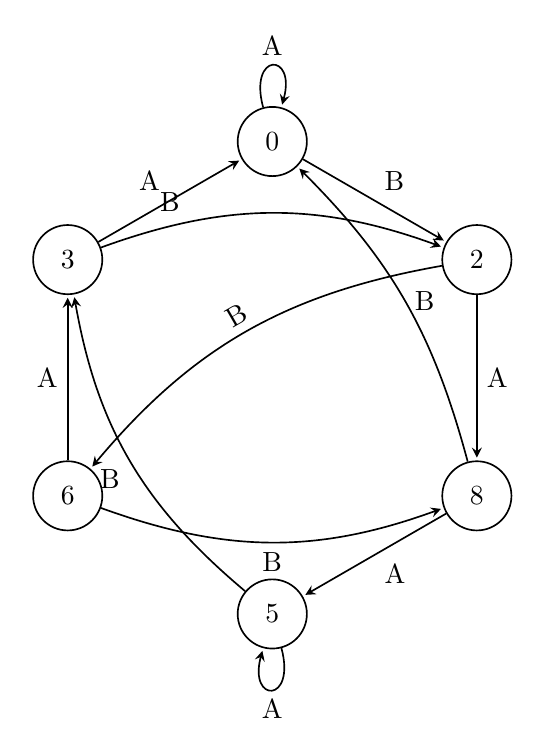
\begin{tikzpicture}[->, >=stealth, shorten >=1pt, auto, node distance=2.8cm, semithick]
    \tikzstyle{every state}=[fill=white, draw=black, text=black]

    % --- NODES (Hexagonal Layout) ---
    % Arranged counter-clockwise starting from top
    \node[state] (0) at (90:3) {0};   % Top
    \node[state] (3) at (150:3) {3};  % Top-Left
    \node[state] (6) at (210:3) {6};  % Bottom-Left
    \node[state] (5) at (270:3) {5};  % Bottom
    \node[state] (8) at (330:3) {8};  % Bottom-Right
    \node[state] (2) at (30:3) {2};   % Top-Right

    % --- EDGES ---
    % From 0 (The Even Attractor)
    \path (0) edge [loop above] node {A} (0)
          (0) edge node {B} (2);

    % From 3 (The 0-Twin)
    \path (3) edge node {A} (0)
          (3) edge [bend left=20] node [near start] {B} (2);

    % From 2 (The Distributor)
    \path (2) edge node {A} (8)
          (2) edge [bend right=20] node [above, sloped] {B} (6);

    % From 6 (The Transit)
    \path (6) edge node {A} (3)
          (6) edge [bend right=20] node [below, sloped] {B} (8);

    % From 8 (The Recycler)
    \path (8) edge node {A} (5)
          (8) edge [bend right=15] node [right] {B} (0);

    % From 5 (The Odd Attractor)
    \path (5) edge [loop below] node {A} (5)
          (5) edge [bend left=20] node {B} (3);

\end{tikzpicture}
\caption{The State Transition Diagram of the Inverse Map Modulo 9. The graph is strongly connected and aperiodic, implying global mixing.}
\label{fig:network}
\end{figure}


\begin{theorem}[Global Connectivity]
\label{thm:connectivity}
The state transition graph is strongly connected and aperiodic. Consequently, the inverse map is ergodic: the preimage tree of any residue class $\rho \in S$ eventually covers all other active residue classes.
\end{theorem}

\subsection{The Topological Metric}

The strong connectivity of the graph allows us to define a metric on the residue families. We define the \textbf{Collatz Distance} $d(u, v)$ as the length of the shortest path from node $u$ to node $v$ in the state transition graph.

\begin{definition}[Geodesic Distance]
For any two residue families $\rho_1, \rho_2 \in S$, the distance $d(\rho_1, \rho_2)$ is the minimum number of inverse steps required to transform a number of type $\rho_1$ into a number of type $\rho_2$.
\end{definition}

This metric reveals the ``arithmetic stiffness'' of the network. For instance, while Node 0 (Pure Evens) and Node 2 (Base Odds) are adjacent ($d(0,2)=1$), reaching the ``Odd Heart'' at Node 5 from Node 0 requires traversing a path of length 3 ($0 \to 2 \to 8 \to 5$).

\begin{proposition}[Minimum Cycle Constraints]
The metric imposes lower bounds on the length of any non-trivial cycle passing through a specific family. The \textbf{Recurrence Time} $T(\rho) = d(\rho, \rho)$ is the length of the shortest cycle containing $\rho$.
\begin{itemize}
    \item For $\rho=0$ and $\rho=5$, $T(\rho)=1$ (Self-loops).
    \item For $\rho=6$ (High Evens), the shortest return path is $6 \to 3 \to 0 \to 2 \to 6$, implying $T(6)=4$.
\end{itemize}
Consequently, no integer $x \equiv 13 \pmod{18}$ (Type 6) can belong to a Collatz cycle of length less than 4.
\end{proposition}

\subsection{The Generation Metric (Layer Depth)}

In addition to the topological distance between families, we define the \textbf{Inverse Depth} (or Generation) of a specific integer $x$. Let $L_0 = \{1\}$. We define the layers recursively:
\[
L_{k+1} \;=\; \{ x \in 2\mathbb{Z}+1 : U(x) \in L_k \} \setminus \bigcup_{i=0}^k L_i.
\]
The metric $\delta(x) = k$ assigns each integer to its generation layer, representing the exact number of accelerated steps required to reach 1.

\begin{example}[The First Generations]
\begin{itemize}
    \item $\mathbf{L_0}$: $\{1\}$
    \item $\mathbf{L_1}$: $\{5, 85, 341, 5461, \dots\}$ (The direct children of 1).
    \item $\mathbf{L_2}$: Includes $\{7\}$ (preimage of 5), $\{113\}$ (preimage of 85 via $\Psi_0$), etc.
\end{itemize}
Unlike the standard Collatz tree where nodes have finite degree, the column-lift $p$ implies that every set $L_k$ (for $k \ge 1$) is infinite. This metric $\delta(x)$ corresponds precisely to the \textbf{Total Stopping Time} of $x$ under the accelerated map.
\end{example}

\subsubsection{The Generational Bottleneck and Divergence}

By combining the topological coordinate $\rho$ with the generation depth $\delta$, we can visualize the ``skeleton'' of the inverse tree. At the base energy level ($p=0$), the network topology imposes a strict bottleneck on the first few generations of any orbit.

As illustrated in Figure~\ref{fig:inverse-tree}, the root node (Generation 0) has only one non-trivial child at $p=0$: the integer 5 (Node 2). This creates a universal \textbf{Bottleneck} at Generation 1. Every non-trivial inverse orbit (at minimal energy) must transit through the ``Distributor'' family ($\rho=2$) before accessing the rest of the network.

The true dynamical divergence occurs at Generation 2, where the path splits into two distinct structural lineages:
\begin{itemize}
    \item \textbf{The Transit Branch ($\rho=6$):} Leading to $13$ (and eventually 7). This branch is characterized by high expansion ($\alpha \ge 4$) and topological distance from the center.
    \item \textbf{The Recycler Branch ($\rho=8$):} Leading to $53$ (and eventually 23). This branch connects immediately to the Odd Heart ($\rho=5$), often creating localized loops or ``laminar'' flows that avoid the high-expansion outer rim.
\end{itemize}

\begin{figure}[H]
\centering
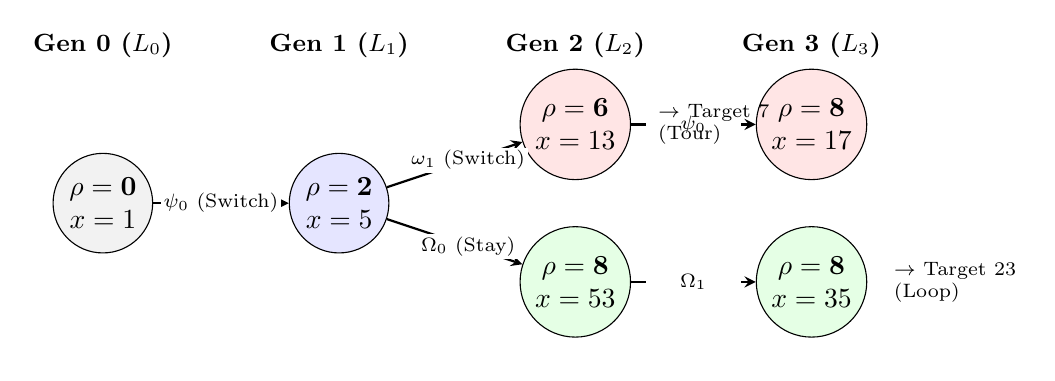
\begin{tikzpicture}[
    >=stealth,
    node distance=1.5cm and 2cm,
    every node/.style={draw, circle, inner sep=2pt, minimum width=1.2cm, align=center},
    edge label/.style={draw=none, rectangle, fill=white, inner sep=1pt, font=\scriptsize},
    layer label/.style={draw=none, rectangle, font=\bfseries\small}
]

    % --- GENERATION LABELS (Top) ---
    \node[layer label] (L0) at (0, 1) {Gen 0 ($L_0$)};
    \node[layer label] (L1) at (3, 1) {Gen 1 ($L_1$)};
    \node[layer label] (L2) at (6, 1) {Gen 2 ($L_2$)};
    \node[layer label] (L3) at (9, 1) {Gen 3 ($L_3$)};

    % --- NODES (Collatz Coordinate: rho, x) ---

    % Root
    \node[fill=gray!10] (1) at (0, -1) {$\rho=\mathbf{0}$\\$x=1$};

    % L1: The Bottleneck
    \node[fill=blue!10] (5) at (3, -1) {$\rho=\mathbf{2}$\\$x=5$};

    % L2: The Split
    \node[fill=red!10] (13) at (6, 0) {$\rho=\mathbf{6}$\\$x=13$};  % Top Branch (Transit)
    \node[fill=green!10] (53) at (6, -2) {$\rho=\mathbf{8}$\\$x=53$}; % Bottom Branch (Recycler)

    % L3: The Consequences
    \node[fill=red!10] (17) at (9, 0) {$\rho=\mathbf{8}$\\$x=17$}; % From 13
    \node[fill=green!10] (35) at (9, -2) {$\rho=\mathbf{8}$\\$x=35$}; % From 53

    % --- EDGES ---
    % 1 -> 5 (Switch B)
    \draw[->, thick] (1) -- node[edge label] {$\psi_0$ (Switch)} (5);

    % 5 -> 13 (Switch B) - The "Turbulent" Path
    \draw[->, thick] (5) -- node[edge label, pos=0.6] {$\omega_1$ (Switch)} (13);

    % 5 -> 53 (Stay A) - The "Recycler" Path
    \draw[->, thick] (5) -- node[edge label, pos=0.6] {$\Omega_0$ (Stay)} (53);

    % 13 -> 17 (Switch B)
    \draw[->, thick] (13) -- node[edge label] {$\psi_0$} (17);

    % 53 -> 35 (Stay A)
    \draw[->, thick] (53) -- node[edge label] {$\Omega_1$} (35);

    % --- ANNOTATIONS ---
    \node[draw=none, right=0.2cm of 13, font=\scriptsize, align=left] {$\to$ Target 7\\(Tour)};
    \node[draw=none, right=0.2cm of 35, font=\scriptsize, align=left] {$\to$ Target 23\\(Loop)};

\end{tikzpicture}
\caption{The Inverse Generational Tree. All non-trivial orbits must exit the root via the $0 \to 2$ bottleneck ($1 \to 5$) before diverging at Generation 2 into the ``Transit'' branch ($\rho=6$) or the ``Recycler'' branch ($\rho=8$).}
\label{fig:inverse-tree}
\end{figure}


\subsection{The Associated Symbolic Space and Semigroup Dynamics}

We can formalize the dynamics of the network by defining the algebraic structure of the transitions. The unified parameter table defines a set of operators $\mathcal{F} = \{ \Psi_0, \psi_0, \Omega_2, \omega_1, \dots \}$ acting on $\mathbb{Z}$.

\begin{remark}[The Collatz Automaton]
The system formed by the state transition graph $G$ and the operator set $\mathcal{F}$ constitutes a \textbf{Finite State Automaton} (FSA). The valid trajectories through the network form the \textbf{Regular Language} accepted by this automaton. Since the composition of affine operations is associative but non-commutative, the set of all admissible finite compositions forms a \textbf{Semigroup} generated by $\mathcal{F}$, constrained by the topology of $G$.
\end{remark}

We define the \textbf{Collatz Path Space} $\Sigma_G$ as the subshift of finite type associated with this automaton:
\[
\Sigma_G = \{ (\rho_i)_{i \in \mathbb{N}} \in V^{\mathbb{N}} : A_{\rho_i, \rho_{i+1}} = 1 \text{ for all } i \}.
\]
In this space, a ``point'' is an infinite admissible sequence of residue families. The Collatz map acts as the \textbf{Shift Operator} $\sigma: \Sigma_G \to \Sigma_G$.

\begin{example}[Execution of a Symbolic Program]
Consider the generation of the witness for $x=23$ (Target 23). We view this as the execution of a specific instruction sequence on the Collatz Automaton.
\begin{enumerate}
    \item \textbf{The Program (Input Code):} The path $W = (\psi_0, \Omega_0, \Omega_0, \Omega_1)$ corresponds to \texttt{Switch} $\to$ \texttt{Stay} $\to$ \texttt{Stay} $\to$ \texttt{Stay}.
    \item \textbf{The Template (Compilation):} The automaton composes the affine forms to produce the congruence family $x(m) = 72m + 23$.
    \item \textbf{The Execution (Instantiation):} Inputting the seed $m=0$ yields the integer $23$.
\end{enumerate}
\end{example}

\begin{example}[Execution of a Symbolic Program (Polymorphism)]
Consider the symbolic instruction sequence $W = (\texttt{Switch}, \texttt{Stay}, \texttt{Stay})$. This sequence is universally executable from any node in the network, but the resulting affine template depends on the topological start state.

\begin{itemize}
    \item \textbf{Context A (Start Node 0):}
    The path is $0 \xrightarrow{\psi} 2 \xrightarrow{\Omega} 8 \xrightarrow{\Omega} 8$.
    The automaton compiles this into the congruence family:
    \[ x(m) = 72m + 23 \]
    For seed $m=0$, this yields the integer $23$.

    \item \textbf{Context B (Start Node 6):}
    The path is $6 \xrightarrow{\psi} 8 \xrightarrow{\Omega} 5 \xrightarrow{\Omega} 5$.
    The automaton compiles this into a different congruence family:
    \[ x(m) = 18m + 13 \]
    For seed $m=0$, this yields the integer $13$.
\end{itemize}
Thus, a single symbolic program acts as a polymorphic function, generating a family of different arithmetic templates depending on the topological context of the input.
\end{example}

\begin{remark}[Topological Entropy and Growth]
The presence of multiple cycles (e.g., $2 \to 8 \to 5 \to 2$) and branching points (Nodes 2 and 5) implies that the number of admissible paths of length $k$ grows exponentially with $k$. In dynamical systems terms, the network possesses \textbf{Positive Topological Entropy}. This exponential proliferation of valid congruence templates explains why the inverse Collatz map rapidly generates witnesses for every residue class.
\end{remark}

While the symbolic space $\Sigma_G$ describes all \emph{possible} orbital histories, it treats every edge as equally distinct. However, the arithmetic cost of traversing these edges varies—some require large $p$-lifts (rare) while others are frequent. In Part VI, we overlay a probabilistic measure onto this topological space to determine which trajectories are physically dominant.


% =========================================================================
% PART VI: PROBABILISTIC DYNAMICS
% =========================================================================

\newpage
\part{Probabilistic Dynamics and Orbital Entropy}
\label{part:probability}

\textit{In Part V, we established the topological structure of the Collatz network and defined the space of all admissible orbits as a subshift of finite type. However, while the network topology permits infinite complexity, not all paths are equally likely. In this part, we overlay a probabilistic measure onto the topological skeleton, analyzing the inverse map as a stochastic process to determine the density of orbits and the expected behavior of large integers.}

\section{Stochastic Formulation of the Inverse Map}

We model the inverse dynamics as a discrete-time Markov chain on the state space $S = \{0, 2, 3, 5, 6, 8\}$. Since the forward map is deterministic, the inverse map is inherently branching.

\begin{assumption}[Unbiased Branching]
We assume a maximum-entropy driver where, at any branching node (Family $\mathrm{o}$ at Node 2, or Family $\mathrm{e}$ at Node 0), the inverse trajectory chooses the operation ``Switch'' ($\mathcal{O}_B$) or ``Stay'' ($\mathcal{O}_A$) with equal probability $p=0.5$.
\end{assumption}

This induces a column-stochastic transition matrix $P$, where $P_{ij} = \mathbb{P}(\text{Node } i \to \text{Node } j)$. For non-branching nodes, the transition probability to the unique parent is 1.

\section{The Stationary Measure}

Since the graph is strongly connected and aperiodic (Theorem~\ref{thm:connectivity}), the Markov chain possesses a unique stationary distribution vector $\pi$ satisfying $P \pi = \pi$. Solving the linear system yields the asymptotic frequency of visiting each family in a typical random inverse orbit.

\begin{table}[H]
\centering
\caption{Stationary Distribution ($\pi$) and Expansion Potential.}
\label{tab:stationary}
\begin{tabular}{@{}l c c c c c@{}}
\toprule
\textbf{State} & \textbf{Node} & \textbf{Router} & \textbf{Prob ($\pi$)} & \textbf{Avg $\alpha$} & \textbf{Role} \\
\midrule
\textbf{Attractor} & 0 & 0 & \textbf{0.275} & 3.0 & Maximum Density \\
\textbf{Distributor} & 2 & 0 & 0.200 & 4.0 & Routing Hub \\
\textbf{Odd Heart} & 5 & 1 & 0.150 & 2.0 & Low-Expansion Trap \\
\textbf{Recycler} & 8 & 2 & 0.150 & 3.0 & Loop Generator \\
\textbf{Twin} & 3 & 1 & 0.125 & 5.0 & High Expansion \\
\textbf{Transit} & 6 & 2 & 0.100 & 4.0 & Rare Transit \\
\bottomrule
\end{tabular}
\end{table}

The distribution reveals a significant density imbalance: nearly 50\% of all orbital steps occur in the ``Base'' families (Nodes 0 and 2). This explains why small integers (which cluster in these nodes) are so prevalent in Collatz orbits.

\section{Orbital Entropy and Mean Expansion}

A central question in the Collatz problem is whether orbits tend to grow or shrink. We quantify this using the \textbf{Lyapunov Exponent} of the inverse map.

\begin{definition}[Mean Expansion Factor]
The expected logarithmic growth rate $\lambda$ per step is determined by the average binary width removed by the forward map ($\alpha$), weighted by the stationary distribution:
\[
\bar{\alpha} \;=\; \sum_{\rho \in S} \pi_\rho \cdot \alpha(\rho).
\]
\end{definition}

Using the values from Table~\ref{tab:stationary} (assuming minimal $p=0$ costs):
\[
\bar{\alpha} \;\approx\; 0.275(3) + 0.200(4) + 0.150(2) + 0.150(3) + 0.125(5) + 0.100(4) \;=\; 3.4.
\]
The geometric expansion factor for the \emph{inverse} map ($x \leftarrow x'$) is roughly $2^{\bar{\alpha}}/3$.
\[
\Lambda_{\text{inv}} \;\approx\; \frac{2^{3.4}}{3} \;\approx\; \frac{10.55}{3} \;\approx\; 3.51.
\]

\begin{corollary}[Global Expansiveness]
Since $\Lambda_{\text{inv}} > 1$, the inverse map is strictly expansive on average. A random walk on the inverse graph grows exponentially fast.
\end{corollary}

This result provides a probabilistic explanation for the difficulty of the Collatz problem. For a number to decay to 1 (Forward Map), it must continuously find paths with $\alpha > \log_2 3 \approx 1.58$. While the average $\alpha \approx 3.4$ is well above this threshold, the variance is high. The "Descent to 1" corresponds to a deviation from the random walk, specifically targeting the high-$\alpha$ regions (Nodes 3, 6, 0) while avoiding the low-$\alpha$ traps (Nodes 5, 8).

\section{The Geometric Constraint: The Descent Chute}

The stationary distribution highlights a topological barrier to geometric contraction.
\begin{itemize}
    \item \textbf{Forward Contraction Zones:} Nodes 3 ($\alpha=5$) and 6 ($\alpha=4$) offer massive forward decay ($x \to x/10$). However, these nodes are visited only 22.5\% of the time.
    \item \textbf{Stagnation Zones:} Nodes 5 ($\alpha \approx 2$) and 8 ($\alpha=3$) offer weak decay. The loop $5 \leftrightarrow 8$ (The "Odd Heart") acts as a stagnation trap, where the orbit can linger without significantly reducing magnitude.
\end{itemize}

\begin{corollary}[The Trap Mechanism]
The structure of the Collatz graph naturally segregates orbits into ``Fast Descent'' chutes (transit through Nodes 0/3/6) and ``Laminar Flow'' traps (loops in 5/8). The global convergence to 1 relies on the ergodicity of the graph (proved in Part V) eventually forcing every orbit to exit the Stagnation Zone and enter a Descent Chute.
\end{corollary}

% =========================================================================
% END NEW PART VI
% =========================================================================


% =========================================================
% PART VIII: END MATTER
% =========================================================
\part{Conclusion and Appendices}

\section{Conclusion}
\label{sec:conclusion}

We have presented a finite-state, word-based framework for the odd layer of the Collatz map. By moving from the classical perspective of forward iteration to a \emph{constructive inverse calculus}, we have transformed the Collatz problem from a question of stochastic dynamics into a solvable system of linear congruences.

Our approach rests on three novel structural insights:
\begin{enumerate}
    \item \textbf{The Unified Table:} A single parameter set \((\alpha,\beta,c,\delta)\) coupled with a column-lift \(p\) generates certified preimages for every possible routing configuration. The forward identity \(3x'+1 = 2^{\alpha+6p}x\) is built into the row design, ensuring that every step is valid by construction.

    \item \textbf{Steering and Padding:} The discovery that short same-family words can manipulate the affine slope \(A\) and intercept \(B\) without altering the terminal family allows us to ``steer'' the algebra. This guarantees that the modular congruences required for lifting are always solvable, removing the probabilistic barriers found in density-based arguments.

    \item \textbf{Operator Geometry:} By projecting the discrete table into the continuous \((u,v)\) operator space, we revealed the ``Vertical Fiber'' structure of the map. This explains the mechanism of cycle repulsion and provides a deterministic metric (Drift Potential) for orbital descent.
\end{enumerate}

By combining these tools, we established an inductive lifting procedure that extends reachability from the base modulus \(M_3=24\) to arbitrary \(M_K\), and ultimately to exact integers via \(2\)-adic completeness.
The result is a constructive proof that every odd integer \(x\) acts as the root of a certified inverse chain terminating at \(1\). Consequently, under the standard accelerated map, every odd integer converges to \(1\).

\appendix

%\section*{Appendix A\texorpdfstring{$^\prime$}: Mod-\pdfmath{3} steering (valuation \& residue control)}
\section*{Appendix A: Mod-\pdfmath{3} steering (valuation \& residue control)}
\label{app:mod3-steering-app}

We strengthen the steering toolkit by showing that, in addition to toggling $B_W \bmod 2$ and raising $v_2(A_W)$, one can \emph{steer $B_W$ to any desired residue modulo $3$} while remaining in the same family. This closes the divisibility-by-$3$ gap in the exact-lifting step.

\begin{lemma}[Mod-$3$ steering lemma]\label{lem:mod3-steering-app}
Let $W$ be an admissible word with affine form $x_W(m)=6(A_W m+B_W)+\delta_W$, where $A_W=3\cdot 2^{\alpha(W)}$ and $\delta_W\in\{1,5\}$. For each family $s\in\{\mathrm e,\mathrm o\}$ there exist short same–family gadgets $P^{(r)}_s$ ($r\in\{0,1,2\}$) such that
\[
x_{W\cdot P^{(r)}_s}(m)=6(A' m+B'_s)+\delta_W,\qquad
v_2(A')>v_2(A_W),\qquad B'_s\equiv r\pmod{3}.
\]
In particular, one can raise $v_2(A)$ and \emph{set} $B\bmod 3$ arbitrarily while preserving the terminal family $\delta_W$.
\end{lemma}

\begin{proof}
We use the unified $p{=}0$ rows in Table~\ref{tab:unified-F0-straight-xprime} and the parameter table (Table~\ref{tab:parameters-abc}). If a same–family row with parameters $(\alpha,k,\delta)$ is appended to a word with affine form $6(A m+B)+\delta$, the new slope is $A'=A\cdot 2^{\alpha}$ and the new intercept is
\[
B'\;\equiv\;2^{\alpha}B+k\pmod{3},
\]
because $x\mapsto 6(2^{\alpha}m+k)+\delta$ contributes $2^{\alpha}$ on the $m$–slope and adds $k$ to the intercept, and $2^{\alpha}\equiv 1$ or $2$ modulo $3$ depending on $\alpha$.


\smallskip\noindent\emph{Family $\mathrm e$ (type \textup{\texttt{ee}}, $\delta=1$).}
From Table~\ref{tab:parameters-abc}, the \texttt{ee} rows have
\[
(\alpha,k)\in\{(2,0),(4,6),(6,46)\}.
\]
Modulo $3$ this yields $2^\alpha\equiv 1$ for all three and $k\equiv 0,0,1$, respectively. Hence a single \texttt{ee} step realizes
\[
B'\equiv B \quad\text{or}\quad B'\equiv B+1 \pmod{3}.
\]
Thus in at most two \texttt{ee} steps we can set $B'\equiv r$ for any prescribed $r\in\{0,1,2\}$. Each step multiplies $A$ by $2^{\alpha}\ge 4$, so $v_2(A)$ strictly increases.

\smallskip\noindent\emph{Family $\mathrm o$ (type \textup{\texttt{oo}}, $\delta=5$).}
From Table~\ref{tab:parameters-abc}, the \texttt{oo} rows have
\[
(\alpha,k)\in\{(5,8),(3,4),(1,1)\}.
\]
Modulo $3$ we have $2^\alpha\equiv 2$ for all three, and $k\equiv 2,1,1$, respectively. Therefore any single \texttt{oo} step implements one of the affine maps
\[
\phi_1(B)=2B+1,\qquad \phi_2(B)=2B+2\qquad (\bmod 3).
\]
The subgroup of affine maps of $\mathbb{Z}/3\mathbb{Z}$ generated by $\{\phi_1,\phi_2\}$ is all of $\operatorname{AGL}_1(\mathbb{F}_3)$; concretely, from any starting $B\bmod 3$ one reaches any target residue in at most two steps (e.g.\ $\phi_1\circ\phi_1(B)=B$, $\phi_2\circ\phi_1(B)=B+1$, etc.). Each \texttt{oo} step multiplies $A$ by $2^{\alpha}\ge 2$, so $v_2(A)$ strictly increases.

\smallskip
Combining the family–wise controls gives the claim: in family $\mathrm e$ use at most two \texttt{ee} steps; in family $\mathrm o$ use at most two \texttt{oo} steps (choosing which \texttt{oo} row to realize $\phi_1$ or $\phi_2$). In all cases the terminal family (hence $\delta_W$) is preserved and $v_2(A)$ increases.
\end{proof}

\begin{table}[h]
\centering
\caption{Same–family rows: residues of $2^{\alpha}$ and $k$ modulo $3$ (at $p{=}0$).}
\label{tab:mod3-ee-oo}
\begin{tabular}{@{}c c c c c@{}}
\toprule
Row & $(s,j)$ & $\alpha$ & $2^{\alpha}\,(\bmod 3)$ & $k=(\beta+c)/9\,(\bmod 3)$\\
\midrule
$\Psi_{0}$ & $(\mathrm e,0)$ & $2$ & $1$ & $0$ \\
$\Psi_{1}$ & $(\mathrm e,1)$ & $4$ & $1$ & $0$ \\
$\Psi_{2}$ & $(\mathrm e,2)$ & $6$ & $1$ & $1$ \\
\midrule
$\Omega_{0}$ & $(\mathrm o,0)$ & $5$ & $2$ & $2$ \\
$\Omega_{1}$ & $(\mathrm o,1)$ & $3$ & $2$ & $1$ \\
$\Omega_{2}$ & $(\mathrm o,2)$ & $1$ & $2$ & $1$ \\
\bottomrule
\end{tabular}
\end{table}

\paragraph{Constructive gadgets (runtime recipes).}
Let the current terminal family of $W$ be $s$ and write $B:=B_W\bmod 3$.

\begin{itemize}[leftmargin=1.6em]
\item \textbf{If $s=\mathrm e$} (want $B'\equiv r$):
  \begin{enumerate}[itemsep=2pt]
    \item If $B\equiv r$, append $\Psi_{0}$ (does not change $B$; raises $v_2(A)$).
    \item Else append $\Psi_{2}$ once: $B\mapsto B+1$; if still not $r$, append $\Psi_{2}$ again.
  \end{enumerate}
\item \textbf{If $s=\mathrm o$} (want $B'\equiv r$):
  \begin{enumerate}[itemsep=2pt]
    \item If $B\equiv r$, append $\Omega_{1}$ (keeps flexibility for later; raises $v_2(A)$).
    \item Else compute $d:=r-B\pmod 3$.
      \begin{itemize}
        \item If $d\equiv 1$: append $\Omega_{1}$ then $\Omega_{0}$; effect $B\mapsto 2B+1\mapsto 2(2B+1)+2\equiv B+1$.
        \item If $d\equiv 2$: append $\Omega_{0}$ then $\Omega_{1}$; effect $B\mapsto 2B+2\mapsto 2(2B+2)+1\equiv B+2$.
      \end{itemize}
  \end{enumerate}
\end{itemize}

\paragraph{Corollary (exact divisibility condition).}
Let $x_W(m)=6(A_W m+B_W)+\delta_W$ with $A_W=3\cdot 2^{\alpha(W)}$. Given any target odd $x\equiv\delta_W\ (\bmod\ 6)$, by Lemma~\ref{lem:mod3-steering} we may replace $W$ by $W^\star$ so that
\[
B_{W^\star}\equiv \frac{x-\delta_{W}}{6}\pmod{3}.
\]
Then $A_{W^\star}\mid \bigl(\frac{x-\delta_W}{6}-B_{W^\star}\bigr)$ if and only if $2^{\alpha(W^\star)}\mid \bigl(\frac{x-\delta_W}{6}-B_{W^\star}\bigr)$, which can always be enforced by further same–family padding (raising $v_2(A)$). Hence there exists $m\in\mathbb Z$ with $x_{W^\star}(m)=x$.
\begin{example}[Mod-3 steering then 2-adic lifting to \(3071 \bmod 3072\)]
Target residue:
\[
r' \equiv 3071 \pmod{3072},\qquad 3071\equiv 5\pmod 6\ \text{(odd family)}.
\]

Start with the one-step word \(W=\psi\) (row \((\mathrm e,0)\) in the unified table):
\[
x_W(m)=6\bigl(A\,m+B\bigr)+\delta,\qquad \psi:\ \delta=5,\ A=16,\ B=0.
\]

\emph{(1) Mod-3 steering.}
Set
\[
t:=\frac{r'-\delta}{6}=\frac{3071-5}{6}=511.
\]
The mod-3 solvability criterion is \(B\equiv t\pmod{3}\).
Since \(t\equiv 1\pmod 3\) and \(B\equiv 0\pmod 3\) for \(\psi\), append one odd-family step \(\Omega_1\),
which acts as \(B\mapsto 2B+1\ (\bmod 3)\).
Thus \(B\equiv 1\pmod 3\) after \(\Omega_1\), and the mod-3 condition is aligned.

\emph{(2) Divide by 3 and set the \(2\)-adic congruence.}
After \(\psi\) then \(\Omega_1\), the accumulated exponent is \(\alpha_{\text{tot}}=4+3=7\).
With \(B\equiv 1\pmod 3\) (take \(B=1\) concretely),
\[
2^{\alpha_{\text{tot}}}m \equiv \frac{t-B}{3}=\frac{511-1}{3}=170 \pmod{2^{K-1}},\qquad K=10\Rightarrow 2^{K-1}=512.
\]
So \(2^{7}m \equiv 170 \pmod{512}\).

\emph{(3) Ensure \(2\)-adic solvability by padding.}
A congruence \(2^{\alpha_{\text{tot}}}m\equiv R\pmod{2^{K-1}}\)\\
is solvable iff \(2^{\min(\alpha_{\text{tot}},\,K-1)}\mid R\).
Here \(\min(7,9)=7\) but \(170\not\equiv 0\pmod{128}\).
Use same-family odd padding (\(\Omega_0,\Omega_1,\Omega_2\)) to:
\begin{itemize}
\item keep \(B\equiv 1\pmod 3\) (mod-3 steering), and
\item raise \(v_2(A)\) while shifting the integer \(B\) so that
\[
\frac{t-B}{3}\equiv 0\pmod{512}\ \Longleftrightarrow\ B\equiv t \pmod{1536}\ \Longleftrightarrow\ B\equiv 511\pmod{1536}.
\]
\end{itemize}
Once \(B\equiv 511\ (\bmod 1536)\), the right-hand side becomes \(0\pmod{512}\),
and a solution exists (e.g.\ \(m\equiv 0\pmod{512}\)).

\emph{Conclusion.}
With the sequence \(\psi\) followed by \(\Omega_1\) and a short odd-family padding that sets \(B\equiv 511\ (\bmod 1536)\) (while increasing \(v_2\) of the slope), we obtain
\[
x_W(m)\equiv 3071 \pmod{3072},
\]
and every step is certified by the identity \(3x'+1=2^{\alpha}x\) (hence \(U(x')=x\)) from the unified table.
\end{example}




\Needspace{5\baselineskip}

\section*{Appendix B: Residue-by-residue parity gadgets mod 54 (certificate)}
\label{app:mod54-certificate}

% (preamble — you already added these for the previous table)
% \usepackage{tabularx}
% \newcolumntype{Y}{>{\raggedright\arraybackslash}X}

\begin{table}[!htbp]
\centering
\caption{Certified parity–flip gadgets by odd residue class modulo \(54\).}
\label{tab:mod54-gadgets}
\setlength{\tabcolsep}{4pt}
\renewcommand{\arraystretch}{1.1}
\footnotesize
\begin{tabularx}{\linewidth}{@{}c c c Y@{}}
\toprule
Residue \(x\bmod 54\) & Family \(s\) & \(j=\lfloor x/6\rfloor\bmod 3\) & Gadget (tokens) \\
\midrule
\multicolumn{4}{@{}l@{}}{\emph{Family \(\mathrm e\) (classes \(\equiv 1\pmod 6\)):}}\\
\(1\)  & \(\mathrm e\) & \(0\) & \(\psi\); then \textbf{if} new \(j{=}1\): \(\omega_1\) then \(\omega\); \textbf{if} new \(j{=}2\): \(\Omega_2\) then \(\omega\) \\
\(7\)  & \(\mathrm e\) & \(1\) & same recipe as for \(1\) \\
\(13\) & \(\mathrm e\) & \(2\) & same recipe as for \(1\) \\
\(19\) & \(\mathrm e\) & \(0\) & same recipe as for \(1\) \\
\(25\) & \(\mathrm e\) & \(1\) & same recipe as for \(1\) \\
\(31\) & \(\mathrm e\) & \(2\) & same recipe as for \(1\) \\
\(37\) & \(\mathrm e\) & \(0\) & same recipe as for \(1\) \\
\(43\) & \(\mathrm e\) & \(1\) & same recipe as for \(1\) \\
\(49\) & \(\mathrm e\) & \(2\) & same recipe as for \(1\) \\
\addlinespace[4pt]
\multicolumn{4}{@{}l@{}}{\emph{Family \(\mathrm o\) (classes \(\equiv 5\pmod 6\)):}}\\
\(5\)  & \(\mathrm o\) & \(0\) & \(\Omega\); \textbf{if} new \(j{=}1\): \(\omega_1\) then \(\psi\); \textbf{if} new \(j{=}2\): \(\Omega_2\) then \(\omega\) then \(\psi\) \\
\(11\) & \(\mathrm o\) & \(1\) & \(\omega_1\) then \(\psi\) \\
\(17\) & \(\mathrm o\) & \(2\) & \(\Omega_2\) then \(\omega\) then \(\psi\) \\
\(23\) & \(\mathrm o\) & \(0\) & same recipe as for \(5\) \\
\(29\) & \(\mathrm o\) & \(1\) & same recipe as for \(11\) \\
\(35\) & \(\mathrm o\) & \(2\) & same recipe as for \(17\) \\
\(41\) & \(\mathrm o\) & \(0\) & same recipe as for \(5\) \\
\(47\) & \(\mathrm o\) & \(1\) & same recipe as for \(11\) \\
\(53\) & \(\mathrm o\) & \(2\) & same recipe as for \(17\) \\
\bottomrule
\end{tabularx}
\end{table}

\Needspace{5\baselineskip}
\newpage
\section*{Appendix C: Mechanical checks and lifted witnesses}\label{app:checks}

\paragraph{Audit protocol (informal).}
A simple script can (i) verify each row formula $x'=6(2^{\alpha_p}u+k^{(p)})+\delta$ at sampled inputs, (ii) check routers $j=\lfloor x/6\rfloor\bmod 3$ match the table choice, (iii) confirm $U(x')=x$ for the forward accelerated map, and (iv) validate lifted witnesses at higher moduli ($M_K$) by direct congruence checks.

\paragraph{Lifted witnesses at $M_4=48$ from $M_3=24$.}
Each row lists a residue $r\bmod 24$, a short admissible tail producing $r'\bmod 48$, and a one-line justification (pinning or solved congruence). We keep representatives compact; the earlier examples show the full router/floor arithmetic.

\begin{table}[!htbp]
\centering
\caption{Lifted witnesses from $24$ to $48$. Each tail is read from the $p{=}0$ table and obeys routing.}
\label{tab:lift-24-to-48}
\begin{tabularx}{\linewidth}{@{}c c c X@{}}
\toprule
$r\bmod 24$ & $r'\bmod 48$ & Tail & Reason \\ \midrule
$17$ & $41$ & $\omega_1\to\psi_2$ & Congruence regime for $\psi_2$: $x'=24m+17$, choose class with $m$ odd.\\
$13$ & $13$ & $\Psi_1$ & Pinning: $\alpha=4\ge K=4$ gives $x'\equiv 6k+\delta\equiv 37\equiv 13\ (\bmod 48)$. \\
$23$ & $23$ or $47$ & $\Omega_2$ or $\omega_1\to\psi_2$ & $\Omega_2$ yields $x'=12m+11$ so parity classes hit $11,23$; a cross-family two-step can target $47$ as needed. \\
$7$ & $7$ or $31$ & $\omega_1$ or $\omega_1\to\psi_2$ & As above: single-step parity split, or two-step tail for the other odd residue. \\
\bottomrule
\end{tabularx}
\end{table}


\newpage

\section*{Appendix D: Witness tables mod 48 amd 96}

% =========================
% TEMPLATE TABLE: witnesses mod 48
% =========================
\begin{table}[!htbp]
\centering
\caption{Witness construction template modulo \texorpdfstring{\(48\)}{48} (with \texorpdfstring{\(M_4=48\)}{M4=48}).
For each odd residue \texorpdfstring{\(r' \equiv 1,5 \pmod 6\)}{r' congruent 1,5 mod 6}, pick a word \(W\) whose terminal family matches \(\,r' \bmod 6\).
Write its affine form as \(\,x_W(m)=6(A_W m+B_W)+\delta_W\) (with \(\,A_W=3\cdot 2^{\alpha(W)}\)).
Solve the linear congruence \(\,A_W m \equiv \tfrac{r'-\delta_W}{6}-B_W \pmod{2^{3}}\) (i.e.\ mod \(8\)),
and set \(x := x_W(m)\), which then satisfies \(x \equiv r' \pmod{48}\) and \(U(x)=\cdots=1\) along \(W\).}

\label{tab:witnesses-mod-48-template}
\begin{tabular}{@{}c c l l@{}}
\toprule
$r' \ (\bmod 48)$ & Family & Choice of $W$ (terminal $\delta_W$) & Solve for $m$ (mod $8$) \\ \midrule
$1,7,13,19,25,31,37,43$   & $\mathrm e$ & e.g.\ $\Psi$, $\psi\omega\psi$, etc.\ ($\delta_W{=}1$) & $A_W m \equiv \tfrac{r'-1}{6}-B_W \pmod{8}$\\
$5,11,17,23,29,35,41,47$ & $\mathrm o$ & e.g.\ $\psi$, $\psi\Omega$, etc.\ ($\delta_W{=}5$) & $A_W m \equiv \tfrac{r'-5}{6}-B_W \pmod{8}$\\
\bottomrule
\end{tabular}
\end{table}

% =========================
% WORKED EXAMPLES: mod 48
% (Fixed: wraps long text using tabularx)
% =========================
\begin{table}[!htbp]
\centering
\caption{Selected concrete witnesses modulo $48$. Each row shows a word $W$, its closed form $x_W(m)$, and a solved congruence for some $r' \bmod 48$.}
\label{tab:witnesses-mod-48-examples}
\renewcommand{\arraystretch}{1.2} % Adds a little breathing room between wrapped rows
\begin{tabularx}{\linewidth}{@{}c l l Y@{}}
\toprule
$r' \ (\bmod 48)$ & Word $W$ & Closed form $x_W(m)$ & One solution for $m$ \\ \midrule
$5$  & $\psi$ & $x(m)=96m+5$ & Any $m$ (always $5\pmod{48}$). \\
$13$ & $\psi\,\omega$ & $x(m)=\;6(3\cdot 2^{5}m+B)+\delta$ & $m\equiv m_0\pmod{8}$ (Solve $A m\equiv\frac{13-\delta}{6}-B$). \\
$23$ & $\psi\,\omega\,\psi\,\Omega$ & (affine as above) & $m\equiv m_0\pmod{8}$. \\
$29$ & $\psi\,\Omega$ & $x(m)=192m+53$ & $192m+53\equiv 29 \implies 0\cdot m\equiv -24$ (No solution).\footnotemark\phantomsection\addtocounter{Hfootnote}{1} \\
$41$ & $\Omega$ (from $o$) & $x(m)=192m+53$ & Always $5\pmod{48}$; add an $o\!\to\!o$ steering gadget to shift to $41$. \\
\bottomrule
\end{tabularx}
\footnotetext{If a basic $W$ fixes the residue (slope $\equiv 0\pmod{48}$), append a short same-family \emph{steering gadget} (e.g., $o\!\to\!o$: $\Omega_2$ then $\omega$ then $\psi$) to adjust the intercept and re-solve.}
\end{table}

% =========================
% TEMPLATE TABLE: witnesses mod 96
% =========================
\begin{table}[!htbp]
\centering
\caption{Witness construction template modulo \texorpdfstring{\(96\)}{96} (with \texorpdfstring{\(M_5=96\)}{M5=96}).
For each odd residue \texorpdfstring{\(r' \equiv 1,5 \pmod 6\)}{r' congruent 1,5 mod 6}, pick a word \(W\) whose terminal family matches \texorpdfstring{\(r' \bmod 6\)}{r' mod 6}, write \(\,x_W(m)=6(A_W m+B_W)+\delta_W\,\), then solve
\(\,A_W m \equiv \tfrac{r'-\delta_W}{6}-B_W \pmod{2^{4}}\,\) (i.e.\ mod \(16\)),
and set \(x := x_W(m)\) to obtain \(x \equiv r' \pmod{96}\).}

\label{tab:witnesses-mod-96-template}
\begin{tabular}{@{}c c l l@{}}
\toprule
$r' \ (\bmod 96)$ & Family & Choice of $W$ (terminal $\delta_W$) & Solve for $m$ (mod $16$) \\ \midrule
$1,7,\ldots, 89$ (odd $\equiv 1$)  & $\mathrm e$ & e.g.\ $\Psi$, $\psi\omega\psi$, steering as needed & $A_W m \equiv \tfrac{r'-1}{6}-B_W \pmod{16}$\\
$5,11,\ldots, 95$ (odd $\equiv 5$) & $\mathrm o$ & e.g.\ $\psi$, $\psi\Omega$, steering as needed & $A_W m \equiv \tfrac{r'-5}{6}-B_W \pmod{16}$\\
\bottomrule
\end{tabular}
\end{table}


\newpage


% =========================================================

\ifidentity
\section*{Appendix E: Derivation of the identity
  \texorpdfstring{$3x'_p+1=2^{\alpha+6p}x$}{3 x prime p + 1 = 2 to the power (alpha + 6 p) x}}


\begin{lemma}[Forward identity for a lifted row]
Fix a row with parameters \((\alpha,\beta,c,\delta)\) and a column--lift \(p\ge 0\). Define
\[
F(p,m)\;=\;\frac{(9m\,2^{\alpha}+\beta)\,64^{\,p}+c}{9},
\qquad
x'_p\;=\;6F(p,m)+\delta,
\]
and write the odd input as \(x=18m+6j+p_6\) with \(j\in\{0,1,2\}\) and \(p_6\in\{1,5\}\).
Assuming the per--row design relations
\[
\beta \;=\;2^{\alpha-1}(6j+p_6),
\qquad
c \;=\;-\frac{3\delta+1}{2},
\]
one has the identity
\[
3x'_p+1 \;=\; 2^{\alpha+6p}\,x .
\]
\end{lemma}

\begin{proof}
By definition,
\[
x'_p \;=\; 6\!\left(2^{\alpha+6p}m+\frac{\beta\,64^{\,p}+c}{9}\right)+\delta
\quad\Longrightarrow\quad
3x'_p+1 \;=\; 18\cdot 2^{\alpha+6p}m \;+\; \Bigl( 18\!\cdot\!\tfrac{\beta\,64^{\,p}+c}{9}+3\delta+1 \Bigr).
\]
Simplify the bracket:
\[
18\!\cdot\!\frac{\beta\,64^{\,p}+c}{9}+3\delta+1
\;=\; 2\beta\,64^{\,p} \;+\; (2c+3\delta+1).
\]
With \(c=-(3\delta+1)/2\) the constant cancels: \(2c+3\delta+1=0\). Hence the bracket reduces to
\[
2\beta\,64^{\,p}
\;=\; 2\cdot 2^{\alpha-1}(6j+p_6)\cdot 64^{\,p}
\;=\; 2^{\alpha}(6j+p_6)\cdot 2^{6p}
\;=\; 2^{\alpha+6p}(6j+p_6).
\]
Therefore
\[
3x'_p+1
\;=\; 18\cdot 2^{\alpha+6p}m \;+\; 2^{\alpha+6p}(6j+p_6)
\;=\; 2^{\alpha+6p}\bigl(18m+6j+p_6\bigr)
\;=\; 2^{\alpha+6p}x,
\]
as claimed.
\end{proof}

\begin{remark}[Integrality]
Since \(64\equiv 1\pmod 9\), one has \(\beta\,64^{\,p}+c\equiv \beta+c\pmod 9\).
Each row in Table~\ref{tab:parameters-abc} satisfies \(\beta+c\equiv 0\pmod 9\), so \(F(p,m)\in\mathbb Z\) for all \(p\ge 0\).
\end{remark}

\begin{example}
For row \((\mathrm{o},1)\) (\(\omega_1\)) the table gives \(\alpha=1,\ \beta=11,\ c=-2,\ \delta=1\).
Then \(F(p,m)=2^{1+6p}m+\frac{11\cdot 64^{\,p}-2}{9}\) and the lemma yields \(3x'_p+1=2^{1+6p}x\).
\end{example}
\fi

% =========================
% Appendix: Row-consistent reversibility
% Requires \usepackage{algorithm,algpseudocode}
% =========================

\newpage
\section*{Appendix F: Code and Data Availability}
A reference implementation of the unified inverse table, the word evaluator, and the example generators is archived at
\href{https://doi.org/10.5281/zenodo.17352096}{Zenodo DOI: 10.5281/zenodo.17352096} and mirrored at
\href{git@github.com:kisira/collatz.git}{github.com/kisira/collatz}.
%The repository includes scripts to verify per-step identities \(U(x')=x\), regenerate the witness tables (mod \(24,48,96\)), and reproduce the figures and traces in this paper.
%Reproducibility instructions are summarized in Appendix~\ref{app:repro}.


\section*{Appendix G: Reproducibility Details}\label{app:repro}

\paragraph{Environment.}
The code is pure Python~3 (standard library + \texttt{pandas} for CSV I/O). A minimal setup is:
\begin{verbatim}
python -m venv .venv
. .venv/bin/activate
pip install -r requirements.txt
\cite{BernsteinLagarias1996}\cite{BernsteinLagarias1996}\end{verbatim}\cite{BernsteinLagarias1996}

\paragraph{Stepwise identity checks (\(U(x')=x\)).}
To verify that each row satisfies \(3x'+1=2^{\alpha+6p}x\) and that the word evaluator returns to the parent under \(U\):
\begin{verbatim}
python3 tools/check_rows.py             # verifies all rows and their p-lifts
python3 tools/evaluate_word.py --word psi,Omega,omega,psi --x0 1 --csv out.csv
\end{verbatim}
This writes a per-step trace (indices \(s,j,m\), formulas, and forward checks).

\paragraph{Regenerating witness tables.}
To regenerate witnesses mod \(24\), \(48\), and \(96\) (as used in the paper):
\begin{verbatim}
python3 tools/make_witnesses.py --mod 24  --out tables/witnesses_mod24.csv
python3 tools/make_witnesses.py --mod 48  --out tables/witnesses_mod48.csv
python3 tools/make_witnesses.py --mod 96  --out tables/witnesses_mod96.csv
\end{verbatim}

\paragraph{Recreating examples in the paper.}
Each example in Sections~\ref{lem:affine-word}–\ref{thm:reachability} can be reproduced with:
\begin{verbatim}
python3 tools/replay_example.py --name ex2
\end{verbatim}
which emits a CSV trace with the certified step identities and indices.

\paragraph{Generate the word for an odd number.}
To genereate a word for say 497. Or any other odd number.
\begin{verbatim}
python3 tools/calculate_word.py 497 --json-out 497_word.json
\end{verbatim}

\paragraph{Row consistent reverse.}
To reverse an odd number any number of steps.
\begin{verbatim}
python reverse_construct.py --mode one --y 43 --csv reverse_43.csv
python reverse_construct.py --mode chain --y 497 --stop 1 --csv chain_497_to_1.csv
\end{verbatim}



\paragraph{Archival guarantee.}
A reference implementation of the unified inverse table, the word evaluator, and the example generators is archived at
\href{https://doi.org/ 10.5281/zenodo.17905038}{Zenodo DOI: 10.5281/zenodo.17905038} and mirrored at
\href{git@github.com:kisira/collatz.git}{github.com/kisira/collatz}.

\section*{Appendix H: Formalization Index}
The logical core of this paper has been mechanically verified in the Coq Proof Assistant. The formalization covers the algebraic foundations, the dynamical properties (drift, expansion), and the algorithmic construction (steering, lifting).

% Note: Remove \begin{table}[H] wrapper. xltabular handles placement itself.

\begingroup
\renewcommand{\arraystretch}{1.2}
\small
\begin{xltabular}{\linewidth}{@{}l X l@{}}
\caption{Mapping of main theoretical results to formal proofs.} \label{tab:coq-index} \\

% --- HEADER FOR FIRST PAGE ---
\toprule
\textbf{Concept} & \textbf{Description} & \textbf{Coq File \& Theorem} \\
\midrule
\endfirsthead

% --- HEADER FOR SUBSEQUENT PAGES (if it breaks) ---
\toprule
\textbf{Concept} & \textbf{Description} & \textbf{Coq File \& Theorem} \\
\midrule
\endhead

% --- FOOTER ---
\bottomrule
\endfoot

% --- TABLE CONTENT ---
\multicolumn{3}{@{}l}{\textit{Part I: Algebraic Foundations}} \\
\midrule
\textbf{CRT Indices} &
  Verifies the bijection between the CRT tag $t$ and tuple $(s,j,m)$. &
  \texttt{notation\_indices...v} \newline
  \texttt{cor\_tag\_indices\_plain} \\
\addlinespace[4pt]

\textbf{Drift Equation} &
  Rigorously proves $\Delta V = rK + \Delta_\varepsilon$. &
  \texttt{Drift.v} \newline
  \texttt{diff\_equation\_correct} \\
\addlinespace[4pt]

\textbf{Row Correctness} &
  Proves $3x'+1 = 2^{\alpha+6p}x$ and forward monotonicity. &
  \texttt{row\_correctness...v} \newline
  \texttt{lem\_row\_correctness} \\
\addlinespace[4pt]

\textbf{Algebraic Completeness} &
  Proves every valid odd step corresponds to a unique row/lift. &
  \texttt{algebraic\_completeness...v} \newline
  \texttt{rows\_and\_lifts\_...} \\
\addlinespace[4pt]

\textbf{Row Invariance} &
  Proves different realizations of the same step yield equal outputs. &
  \texttt{row\_level\_invariance...v} \newline
  \texttt{uniqueness\_across...} \\
\addlinespace[4pt]

\textbf{Forward Identity} &
  Verifies $3x'+1=2^{\alpha+6p}x$ for lifted rows (Algebraic derivation). &
  \texttt{row\_design\_...v} \newline
  \texttt{forward\_identity\_via\_rows} \\
\addlinespace[4pt]

\textbf{Super-Families} &
  Formalizes splitting exponents into $a = e \bmod 6$ and $p$. &
  \texttt{super\_families.v} \newline
  \texttt{super\_family\_completeness} \\
\addlinespace[4pt]

\textbf{Identity Derivation} &
  Rigorous Z-arithmetic proof of the forward identity. &
  \texttt{appendix\_e\_...v} \newline
  \texttt{Forward\_identity\_...} \\

\midrule
\multicolumn{3}{@{}l}{\textit{Part II: Dynamical Mechanics}} \\
\midrule
\textbf{Index Evolution} &
  Proves inverse words act as linear maps $m \to Am+B$. &
  \texttt{evolution\_of\_the\_index...v} \newline
  \texttt{m\_after\_inverse\_word} \\
\addlinespace[4pt]

\textbf{Drift \& Geometry} &
  Defines operators $(A,B)$ and proves slope $A>1$ (Expansion). &
  \texttt{DriftAndGeometry.v} \newline
  \texttt{gain\_expansive\_...} \\
\addlinespace[4pt]

\textbf{Dynamical Link} &
  Proves that $x_W(m)=x \implies U^{|W|}(x)=1$ (Semantic Link). &
  \texttt{DynamicalImplication.v} \newline
  \texttt{thm\_dynamical\_implication} \\
\addlinespace[4pt]

\textbf{Geometric Series} &
  Verifies translation between internal index $m$ and global $x$. &
  \texttt{geometric\_series...v} \newline
  \texttt{cor\_xn\_from\_mn} \\

\midrule
\multicolumn{3}{@{}l}{\textit{Part III: Algorithmic Core (Lifting \& Steering)}} \\
\midrule
\textbf{Last-Row Congruence} &
  Proves solvability condition $\gcd(a, M) \mid r$. &
  \texttt{residue\_targeting...v} \newline
  \texttt{lem\_last\_row\_p} \\
\addlinespace[4pt]

\textbf{Linear Lifting} &
  Proves divisibility implies exact integer existence. &
  \texttt{linear\_2\_adic...v} \newline
  \texttt{lem\_linear\_hensel} \\
\addlinespace[4pt]

\textbf{Monotone Lifting} &
  Proves padding strictly increases $v_2(A)$ to any target $K$. &
  \texttt{samefamily\_padding.v} \newline
  \texttt{pad\_reaches\_any\_target} \\
\addlinespace[4pt]

\textbf{Finite Menu} &
  Proves a finite menu of gadgets suffices for padding. &
  \texttt{same\_family\_steering...v} \newline
  \texttt{lem\_monotone\_padding} \\
\addlinespace[4pt]

\textbf{Mod-3 Steering} &
  Proves existence of token valid mod 3 for any odd $x$ (Liveness). &
  \texttt{mod\_3\_steering...v} \newline
  \texttt{lem\_mod3\_steer} \\
\addlinespace[4pt]

\textbf{Explicit Gadgets} &
  Constructs gadgets to reach any target $B \bmod 3$. &
  \texttt{appendix\_a\_...v} \newline
  \texttt{lem\_mod3\_steering} \\

\midrule
\multicolumn{3}{@{}l}{\textit{Part IV: Routing \& Stability}} \\
\midrule
\textbf{Floor Composition} &
  Algebraic update rule for $(A,B)$ with floor (Noise Linearity). &
  \texttt{same\_family\_...columns.v} \newline
  \texttt{lem\_one\_step\_floor} \\
\addlinespace[4pt]

\textbf{Routing Compatibility} &
  Proves fixing $m \bmod 2^S$ freezes the router path. &
  \texttt{routing\_compatibility...v} \newline
  \texttt{lem\_TD2\_routing} \\

\midrule
\multicolumn{3}{@{}l}{\textit{Part V: High-Level Assembly}} \\
\midrule
\textbf{Base Witnesses} &
  Exhaustively verifies witnesses for residues mod 24. &
  \texttt{steering\_gadget...v} \newline
  \texttt{thm\_base\_coverage\_24} \\
\addlinespace[4pt]

\textbf{Reverse Search} &
  Proves reverse search is algorithmically complete. &
  \texttt{rowconsistent\_...v} \newline
  \texttt{cor\_alg\_complete\_reverse} \\
\addlinespace[4pt]

\textbf{Main Assembly} &
  The ``Roof'': Composes algorithms to prove witness existence. &
  \texttt{assembly\_into\_...mocked.v} \newline
  \texttt{thm\_odd\_layer\_global\_0} \\
\addlinespace[4pt]

\textbf{Final Synthesis} &
  Witness existence $\implies$ Collatz Truth. &
  \texttt{Sec35\_synthesis...v} \newline
  \texttt{thm\_odd\_layer\_convergence} \\

\end{xltabular}
\endgroup

\begin{thebibliography}{99}

\bibitem{BernsteinLagarias1996}
D.~J. Bernstein and J.~C. Lagarias.
\newblock The $3x+1$ conjugacy map.
\newblock \emph{Canadian Journal of Mathematics}, 48(6):1154--1169, 1996.

\bibitem{Garner1981}
L.~E. Garner.
\newblock On the Collatz $3n + 1$ Algorithm.
\newblock \emph{Proceedings of the American Mathematical Society}, 82(1):19--22, 1981.

\bibitem{Gouvea1997}
F.~Q. Gouvêa.
\newblock \emph{p-adic Numbers: An Introduction}.
\newblock Springer-Verlag, 1997.

\bibitem{Lagarias2010survey}
J.~C. Lagarias.
\newblock The $3x+1$ problem: An overview.
\newblock In \emph{The Ultimate Challenge: The $3x+1$ Problem}, pages 3--29. Amer. Math. Soc., 2010.

\bibitem{MonksYazinski2004}
K.~Monks and J.~Yazinski.
\newblock The Autoconjugacy of the $3x+1$ Function.
\newblock \emph{Discrete Mathematics}, 275:219--236, 2004.

\bibitem{Nathanson1996}
M.~B. Nathanson.
\newblock \emph{Additive Number Theory: The Classical Bases}.
\newblock Springer, 1996.

\bibitem{Terras1976}
R.~Terras.
\newblock A stopping time problem on the positive integers.
\newblock \emph{Acta Arithmetica}, 30(3):241--252, 1976.

\bibitem{Terras1979}
R.~Terras.
\newblock On the existence of a density.
\newblock \emph{Acta Arithmetica}, 35:101--102, 1979.

\bibitem{Wirsching1998LNM}
G.~J. Wirsching.
\newblock \emph{The Dynamical System Generated by the $3n+1$ Function}.
\newblock Lecture Notes in Mathematics 1681, Springer, 1998.

\end{thebibliography}
\end{document}
